%%%%%%%%%%%%%%%%%%%%%%%%%%%%%%%%%%%%%%%%%%%%%%%%%%%%%%%%%
% Niniejszy plik przedstawia przykładowy skład 
% pracy dyplomowej na Wydziale Matematyki PWr. 
% 
% Autorzy: 
% Damian Fafuła
% Michał Kijaczko
% Jakub Michalczak
% Maciej Miśta
% Dagmara Nowak
% Tomasz Skalski
% Wojciech Słomian
%
%% Data utworzenia: 8.05.2018
% Numer wersji: 1
%
% Poniższą formatkę można rozpowszechniać i edytować 
% pod warunkiem zachowania numeru wersji, 
% informacji o autorach i dodaniu informacji 
% o wprowadzonych zmianach.
%
%%%%%%%%%%%%%%%%%%%%%%%%%%%%%%%%%%%%%%%%%%%%%%%%%%%%%%%%%
% Domyślną opcją jest: praca magisterska, język polski.
% W przypadku pracy pisanej w języku angielskim dodajemy 
% opcję [english].
% Dla pracy licencjackiej dodajemy opcję [licencjacka].
% Dla pracy inżynierskiej dodajemy opcję [inzynierska].
% Dopuszczalne są podwójne opcje, np. [licencjacka, english].
% Opcje dodajemy w kwadratowym nawiasie przy \documentclass.
%
%
%%%%%%%%%%%%%%%%%%%%%%%%%%%%%%%%%%%%%%%%%%%%%%%%%%%%%%%%%
\documentclass[magisterska, english]{pwr_wmat_praca_dyplomowa}
%%%%%%%%%%%%%%%%%%%%%%%%%%%%%%%%%%%%%%%%%%%%%%%%%%%%%%%%%
%              DANE DO PRACY
%
% W przypadku pracy dyplomowej w języku angielskim nie jest konieczne 
% wypełnianie pól: \tytul{}, \kierunek{}, \specjalnosc{}, 
%                  \streszczenie{}, \slowakluczowe{}.
%%%%%%%%%%%%%%%%%%%%%%%%%%%%%%%%%%%%%%%%%%%%%%%%%%%%%%%%%
%
% Imię i nazwisko autora
\autor{Piotr Florek}
%
% Tytuł pracy dyplomowej 
\tytul{Tytuł pracy dyplomowej} 
\tytulang{Comparative analysis of gradient boosting algorithms used for classification problems}
%
% Tytuł / stopień / imię i nazwisko opiekuna
\opiekun{dr Adam Zagdański}
%
% Kierunek studiów wybieramy spośród następujących:
% 1) Matematyka
% 2) Matematyka i Statystyka
% 3) Matematyka stosowana
\kierunekstudiow{Matematyka stosowana}
%
% Kierunek studiów po angielsku wybieramy spośród następujących:
% 1) Mathematics
% 2) Mathematics and Statistics
% 3) Applied Mathematics
\kierunekstudiowang{Applied Mathematics}
%
% Specjalność wybieramy spośród następujących: 
% KIERUNEK: Matematyka
% 1) Matematyka teoretyczna,
% 2) Statystyka matematyczna,
% 3) Matematyka finansowa i ubezpieczeniowa,
%
% KIERUNEK: Matematyka i Statystyka
% 4) Matematyka,
% 5) Statystyka i analiza danych, 
%
% 6) -- (w przypadku braku specjalizacji).
\specjalnosc{Data engineering} 
%
% Specjalność w języku angielskim wybieramy spośród następujących:
% KIERUNEK: Matematyka
% 1) Theoretical Mathematics,
% 2) Mathematical Statistics,
% 3) Financial and Actuarial Mathematics,
%
% KIERUNEK: Matematyka i Statystyka
% 4) Mathematics,
% 5) Statistics and Data Analysis,
%
% KIERUNEK: Applied Mathematics
% 6) Financial and Actuarial Mathematics, 
% 7) Mathematics for Industry and Commerce,
% 8) Computational Mathematics,
% 9) Modelling, Simulation and Optimization.
%
% 10) -- (w przypadku braku specjalizacji).
\specjalnoscang{Data engineering} 
%
% Krótkie streszczenia po polsku i angielsku
% - nie dłuższe niż 530 znaków.
\streszczenie{Tutaj piszemy krótkie streszczenie pracy (nie powinno być dłuższe niż 530 znaków).}
\streszczenieang{Tutaj piszemy krótkie streszczenie pracy w języku angielskim (nie powinno być dłuższe niż 530 znaków).}
%
% Podajemy najważniejsze słowa kluczowe po polsku i angielsku
% - w obu przypadkach, nie więcej niż 150 znaków.
\slowakluczowe{tutaj podajemy najważniejsze słowa kluczowe (łącznie nie powinny być dłuższe niż 150 znaków).}  
\slowakluczoweang{tutaj podajemy najważniejsze słowa kluczowe w języku angielskim (łącznie nie powinny być dłuższe niż 150 znaków)}
%
%
 %%%%%%%%%%%%%%%%%%%%%%%%%%%%%%%%%%%%%%%%%%%%%
\theoremstyle{plain}
\newtheorem{theorem}{Twierdzenie}
\numberwithin{theorem}{chapter}
\newtheorem{lemma}[theorem]{Lemat} 
\newtheorem{corollary}[theorem]{Wniosek}
\newtheorem{fact}[theorem]{Fakt}
\theoremstyle{definition}
\numberwithin{theorem}{chapter}
\newtheorem{definition}[theorem]{Definicja} 
\newtheorem{example}[theorem]{Przykład}
\newtheorem{note}[theorem]{Uwaga}
 %%%%%%%%%%%%%%%%%%%%%%%%%%%%%%%%%%%%%%%%%%%%%
 
\usepackage{polski}
\usepackage{verbatim}
\usepackage{bm}
\usepackage{cases}
%\usepackage[font=small,aboveskip=0pt,skip=1pt]{caption}
%\usepackage[font=small,aboveskip=12pt,skip=12pt]{caption} % zalec
%\usepackage[font=small]{caption} % 10pt domyślnie
\usepackage{graphicx}
\usepackage{footnote}
\usepackage{diagbox}
%\usepackage[table]{xcolor}
\usepackage{lscape}
\usepackage{longtable}
\usepackage{rotating,booktabs}
\usepackage{rotating}
 %%%%%%%%%%%%%%%%%%%%%%%%%%%%%%%%%%%%%%%%%%%%%
 

 %%%%%%%%%%%%%%%%%%%%%%%%%%%%%%%%%%%%%%%%%%%%%
 
\newcommand{\xle}{\leqslant}
\newcommand{\xge}{\geqslant}
\newcommand{\R}{\mathbb{R}}
\newcommand{\gbm}{GBM, XGBoost, LightGBM and CatBoost }
\newcommand{\U}{$\mathcal{U}$}
\newcommand{\logU}{$\log\mathcal{U}$}
 %%%%%%%%%%%%%%%%%%%%%%%%%%%%%%%%%%%%%%%%%%%%%
 
\def\independenT#1#2{\mathrel{\rlap{$#1#2$}\mkern2mu{#1#2}}}
\hypersetup{pdfauthor={Name}}
\DeclareMathOperator{\E}{\mathbb{E}}
\renewcommand{\Pr}{\qopname \relax m{P}}
\raggedbottom 
\makesavenoteenv{tabular}
\makesavenoteenv{table}
 %%%%%%%%%%%%%%%%%%%%%%%%%%%%%%%%%%%%%%%%%%%%%
 
\begin{document}
\frontmatter
\maketitle
\mainmatter
\thispagestyle{empty}
\begin{flushright}
  \null\vfill
  \Large
  \textit{
  Nice.}\\
  \vspace{-1cm}
\end{flushright}

\tableofcontents

\chapter{Introduction}
\section{State-of-the-art}
The concept of boosting has existed for over 30 years. The first discussions about combining several weak learners into a strong one date back to 1984. However, only in 1990 the concept has been proven to be reasonable by Robert E. Schapire \cite{schapire1990}. His work served as a base for further development of the idea of boosting. Consequently, AdaBoost, one of the first boosting algorithms has been introduced in 1996 by Freund and Schapire. It has been designed with classification problems in mind and it quickly became one of the most prominent algorithms available. In fact, in 1996 Leo Breiman, the creator of bagging claimed that AdaBoost with trees is "\emph{best off-the-shelf classifier in the world}” \cite{esl}. In \cite{add_log} a statistical view of boosting has been presented --- AdaBoost has been rederived as a method for
fitting an additive logistic regression model.

Gradient boosting (GBM) was proposed by Jerome H. Friedman in 1999 in \cite{friedman_gbm}. The concept of combining boosting and the method of steepest descent has been thoroughly discussed. Friedman has presented algorithms for various loss functions used for either regression or classification tasks. He also presented some empirical results and recommendations regarding shrinkage (which controls the learning speed) and number of learners. Additionally, improvements to the gradient boosting algorithm in the case of regression tree being the base learner have been shown. 

In \cite{friedman_stoch} Friedman discussed the idea of stochastic gradient boosting. The idea has been inspired by Breiman's work --- during each boosting iteration, the base learner is trained on a subset which is drawn without replacement from the original one. By performing simulations, Friedman has proven that introducing randomness in form of subsampling can substantially increase the performance of the ensemble in regression or classification tasks. The findings obtained by Friedman will be taken into consideration in Section {wyniki}. % referencja do sekcji wynikowej 
Also, the baseline gradient boosting algorithm with subsampling (stochastic GBM) proposed by Friedman will be one of the tested models.

The research on gradient boosting progressed the most in the second decade of the XXI century. Several advancements in technology and enormous increase in computational power led to development of three state-of-the-art GBM implementations: XGBoost \cite{xgboost} which was released first (2014), LightGBM \cite{lightgbm} (2016) and CatBoost \cite{catboost} (2017). Authors of XGBoost \cite{xgboost} proposed many improvements over the gradient boosting algorithm introduced by Friedman \cite{friedman_gbm}, including introduction of regularized learning objective, approximate algorithm for split finding and sparsity-aware split finding. Additionally, authors claimed that XGBoost scales well with big amount of data due to having several computational optimizations (e.g. GPU training or out-of-core computation). Moreover, authors compared the performance of their algorithm to already existing frameworks, including implementation in \emph{R} and scikit-learn \cite{sklearn}. It has been concluded that in classification and learning to rank tasks XGBoost significantly outperforms basic GBM both in terms of AUC score and runtime; in case of one dataset the improvement in the execution time was over ten-fold.

The development process of LightGBM \cite{lightgbm} has been influenced by the implementation of XGBoost. A big emphasis has been put on the computational aspect of LightGBM as it has been stated that the scalability of XGBoost is not satisfactory for high number of samples and features. In \cite{lightgbm} it is mentioned that in the context of gradient boosting implementations, due to increasing data size an accuracy-efficiency trade-off has emerged. To greatly reduce the training time, LightGBM developers proposed two novel algorithms: Gradient-based One-Side Sampling (GOSS) and Exclusive Feature Bundling (EFB) which decrease the time to process all observations and features, respectively.

A thorough comparison of XGBoost and LightGBM has been performed. The datasets which has been used contained millions of samples which really tested the scalability of both methods. Two variants of XGBoost (exact and histogram algorithm) and three variations of LightGBM have been used, however, it has been shown that LightGBM with GOSS and EFB was the fastest and achieved the highest value of AUC score both on sparse and dense datasets. In case of two biggest datasets, LightGBM was faster than XGBoost (with exact greedy splitting algorithm which is used in decision trees) more than 37 and 15 times, respectively while the histogram variant of XGBoost has caused "out of memory" error. The results obtained by the creators of LightGBM clearly indicate that using GOSS and EFB simultaneously will greatly reduce the fitting time of the algorithm without sacrificing the accuracy or AUC score.

While XGBoost \cite{xgboost} and LightGBM \cite{lightgbm} implementations were focused more on the computational aspect of gradient boosting, authors of CatBoost \cite{catboost} have put a big emphasis eliminating so called "the prediction shift". They claimed that it had never been addressed or formally defined before in any GBM implementation, however, it may have a significant impact on the model's performance. Authors show theoretical explanation the prediction shift phenomena and thus present an Ordered Boosting algorithm which tackles the aforementioned problem by using a permutation based approach. Ordered Boosting has been compared to a non-ordered variant (called Plain boosting) and it has been concluded that addressing the prediction shift yields slightly better results. 

Categorical variables preprocessing is another aspect of CatBoost which has been discussed very thoroughly by the authors. It is claimed that the prediction shift also occurs in case of the aforementioned preprocessing; a novel method of handling categorical variables has been presented. Additionally, a comparison of CatBoost, XGBoost and LightGBM has been shown in \cite{catboost} --- both baseline and tuned models using hyperparameter search have been considered. It has been concluded that across all datasets, CatBoost yielded the most prominent results; the values of both analyzed loss functions was the lowest, although XGBoost and LightGBM performed only slightly worse. What is really interesting is that a baseline Plain version of CatBoost (the one which is very similar to the original gradient boosting implementation introduced in \cite{friedman_gbm}) without having its hyperparameters tuned was better than tuned versions of XGBoost and LightGBM.
The authors also gave detailed description of their experiments. In the comparative analysis of  CatBoost, XGBoost and LightGBM hyperparameter tuning has been performed using bayesian optimization with Tree Parzen Estimators \cite{tpe}. Also, the idea of bayesian search will be taken into consideration in Section \ref{chapter:results}.  % referencja do sekcji z wyn

However, the comparisons of algorithms presented in \cite{lightgbm} and \cite{catboost} might not necessarily be objective. The authors of LightGBM or CatBoost may have chosen such combination of the analyzed datasets and models' hyperparameters subjectively --- it is reasonable to think that they wanted to prove the superiority of their GBM implementations. Therefore, it is crucial to take into the consideration analyses made by impartial researches who are not creators of any of the algorithms. In \cite{competitive_analysis} four algorithms have been compared: XGBoost, LightGBM, CatBoost and SnapBoost. SnapBoost is another state-of-the-art implementation of gradient boosting machines, however, it does not seem to be publicly available. Similarly to the analysis done in \cite{catboost}, both baseline and tuned (using Tree Parzen Estimators) models have been compared. A numerical, categorical, temporal and image datasets have been used. Authors have provided the reader with all search spaces that have been used --- in most cases, basic hyperparameters such as \emph{max\_depth}, \emph{n\_estimators}, \emph{learning\_rate} or regularization ones have been tuned. It has been concluded that XGBoost and SnapBoost were the most consistent in terms of accuracy and fitting time across all four datasets. Also, CatBoost was the most accurate in the case of two datasets, although it was the slowest across three. Additionally, it performed the best on the categorical dataset. LightGBM and SnapBoost needed the least amount of time to be trained. Also, it is said that hyperparameter tuning improved models' performance significantly. Overall, the conclusions indicate that of out of three algorithms: XGBoost, LightGBM and CatBoost one cannot choose the best method which is the fastest and most accurate in all cases.

A significantly more detailed comparative analysis have been presented in \cite{comparative_analysis}. The authors clearly highlighted important hyperparameters of each model. A comparison of random forest, gradient boosting, XGBoost, GOSS LightGBM and Ordered CatBoost has been made. An emphasis has been put on new specific characteristics of algorithms with respect to original GBM: $\gamma$ term in XGBoost, GOSS in LightGBM and a permutation based approach which deals with prediction shift in CatBoost. In \cite{comparative_analysis} a variety across 28 used datasets was substantial --- there were numerical, categorical, sparse and dense datasets. The diversity was also reflected in the sizes, with number of samples ranging from 74 to 19020. The biggest number of features was 60; also, the number of classes varied from 2 to 18.

The authors of \cite{comparative_analysis} have approached hyperparameter tuning in a standard way, namely by using grid search. Authors have given recommendations regarding the choice of hyperparameters to tune --- the number of trees need not to be tuned, it should be set to the highest computationally feasible value; then, learning rate can be tuned. Additionally, it is claimed that in case of XGBoost tuning of randomization parameters: \emph{subsample} \cite{friedman_stoch} and and the number of features selected at each split \emph{colsample\_by\_node} is not needed. It is sufficient to set values of both so that some form of randomization is present.

In \cite{comparative_analysis} it is observed that Ordered CatBoost tuning took the longest despite having the smallest defined search space, however, it is claimed that it scales well as the dataset size increases. Moreover, Ordered CatBoost provided very competitive results without hyperparameter tuning, which suggests that CatBoost might be the best GBM implementation "out of the box" --- both tuned and non-tuned versions yielded very similar results. Also, it is mentioned that LightGBM sometimes performs the best, however, the behaviour is not consistent. On the other hand, base versions of XGBoost and GBM perform generally worse than their tuned counterparts. However, the results presented in \cite{comparative_analysis} were not always statistically significant. 
Authors of \cite{comparative_analysis} have also used an interesting ranking method of the algorithms % referencja
--- it will be also considered in this work. In conclusion, across all datasets there is no such algorithm that performs the best in terms of accuracy or AUC score and fit or tuning time.

In \cite{comparison_of} three GBM implementations: XGBoost, LightGBM and CatBoost have been compared in the context of classification and regression problems. Computations for the analysis have been performed on a personal computer, because most students and researchers do not have the access to more computationally powerful machines (which were used for comparisons in\cite{xgboost}, \cite{lightgbm}, \cite{catboost} \cite{comparative_analysis}, \cite{competitive_analysis}). Apart from comparing accuracy and runtime of the algorithms, authors of \cite{comparison_of} have also taken reliability and ease of use into consideration. In \cite{comparative_analysis} it has been concluded that LightGBM performs the best in terms of accuracy and fitting time; also, it has labeled as easy to use since it is also capable of processing categorical variables. However, it is claimed that all three models: XGBoost, LightGBM and CatBoost still managed to reach state-of-the-art performance level. 

In summary, comparative analyses of gradient boosting algorithms presented in \cite{lightgbm}, \cite{catboost}, \cite{comparative_analysis}, \cite{competitive_analysis} and \cite{comparison_of} lead to a similar conclusion --- a thorough investigation has to be carried out. 

\chapter{Experimental results}\label{chapter:results}
Gradient boosting, XGBoost, LightGBM and CatBoost are highly complex algorithms, thus it is crucial to compare and analyze them on different axes. In this chapter results of several different experiments have been presented:
\begin{enumerate}
    \item Comparison of performance metrics of GBM implementations across real datasets
    \item Analysis of XGBoost regularization hyperparameters
    \item Comparison of categorical variables encodings on the basis of CatBoost
    \item Assessment of feature importances across Gradient boosting, XGBoost, LightGBM and CatBoost. 
\end{enumerate}
\section{Used benchmark datasets}\label{section:real_datasets}
GBM implementations, as well as other Machine Learning algorithms are usually used in practical scenarios, thus it is essential to use real datasets in the comparative analysis. In total, twelve publicly accessible datasets have been considered --- some of them are well known staples in the data science community. Some characterisitcs of the used raw data which will be considered have been presented in Table~\ref{tab:datasets}.
\newpage
\begin{table}[h!] % url do mikromacierzy
\centering
\begin{tabular}{|c|c|c|c|c|}
\hline
\textbf{dataset}  & \textbf{\# samples} & \textbf{\# features} & \textbf{\# classes} & \textbf{type} \\ \hline
adult study\footnote{\url{www.kaggle.com/datasets/wenruliu/adult-income-dataset}}       & 48842              & 13                  & 2                  & mixed         \\ \hline
heart disease\footnote{\url{archive.ics.uci.edu/ml/datasets/Heart+Disease}}     & 303                & 13                  & 2                  & mixed         \\ \hline
amazon\footnote{\url{www.kaggle.com/competitions/amazon-employee-access-challenge/overview}}            & 32769              & 9                   & 2                  & categorical   \\ \hline
mushrooms\footnote{\url{www.kaggle.com/datasets/uciml/mushroom-classification}}           & 8124               & 22                  & 2                  & categorical   \\ \hline
breast cancer\footnote{\url{www.kaggle.com/datasets/uciml/breast-cancer-wisconsin-data}}     & 569                & 30                  & 2                  & numerical     \\ \hline
churn\footnote{\url{www.kaggle.com/datasets/blastchar/telco-customer-churn}}             & 7043               & 20                  & 2                  & mixed         \\ \hline
credit card fraud\footnote{\url{www.kaggle.com/datasets/mlg-ulb/creditcardfraud}} & 30000              & 30                  & 2                  & numerical     \\ \hline
prostate\footnote{\url{url}}          & 102                & 6033                & 2                  & numerical     \\ \hline
leukemia\footnote{\url{url}}          & 72                 & 3571                & 2                  & numerical     \\ \hline
gina agnostic\footnote{\url{www.openml.org/search?type=data&status=active&id=1038}}     & 3468               & 970                 & 2                  & image, sparse \\ \hline
weather\footnote{\url{data.mendeley.com/datasets/4drtyfjtfy/1}}           & 1125               & 2500                & 4                  & image         \\ \hline
IMDB reviews\footnote{\url{www.kaggle.com/lakshmi25npathi/imdb-dataset-of-50k-movie-reviews}}      & 10000              & 10000               & 2                  & NLP, sparse   \\ \hline
\end{tabular}
\caption{Benchmark datasets used for analysis}
\label{tab:datasets}
\end{table}
Variety across datasets summarized in \ref{tab:datasets} is substantial --- they have been chosen mindfully so that the algorithms can be tested in several different scenarios. Raw data varies in number of rows, features (both numerical and categorical), classes and also in the class imbalance and type. Two datasets --- \emph{credit card fraud} and \emph{IMDB reviews} have been downsampled in order to reduce the computational effort; \emph{credit card fraud} originally contains over 27 thousand rows while \emph{IMDB reviews} has exactly 50 thousand reviews. Also, \emph{adult study}, \emph{heart disease} and \emph{churn} datasets contain 7, 3 and 10 categorical features, respectively --- each of them vary in cardinality (its high value can be challenging for decision tree algorithms).

Minor preprocessing of the data has been performed: a redundant feature \emph{education} have been deleted from the \emph{adult study} dataset. Also, numerical features from two out of three unstructured datasets: \emph{weather} and \emph{IMDB reviews} have been extracted. In case of the \emph{weather} database, all images have been resized to 256x256 pixels and converted to grayscale. Then, an area of size 50x50 have been cropped from the center of each picture. Finally, each sample is represented by a vector of length 2500 which contains the values of pixels --- such approach is not perfect, because the geometrical structure of the image is lost, however, in case of many Machine Learning algorithms it is the only one. 

\section{Performance metrics comparison}
In this section, all four GBM implementations: Gradient boosting, XGBoost, LightGBM and CatBoost have been thoroughly compared on all twelve datasets which have been presented in Section~\ref{section:real_datasets}. It was crucial to design a procedure which would allow model selection and model assessment in the most correct way possible.

\subsection{Model selection and assessment}
In applications, the performance of models can be judged and assessed by different criteria, therefore, it was essential to choose appropriate evaluation metrics --- three common ones have been chosen:

\begin{enumerate} % to do sekcji teoretycznej, zostawić tylko nazwy bez enumerate
    \item accuracy --- the fraction of predictions which are correct
    \item f1 score --- the harmonic mean of precision and recall (sensitivity) metrics given by
    \begin{equation}\label{eq:F1}
        F1 = \frac{2}{\frac{1}{precision} + \frac{1}{recall}} = 2\cdot \frac{precision\cdot recall}{precision + recall}.
    \end{equation}
    In the multi-class classification case weighted F1 has been chosen; it calculates the F1 score given by Eq.\eqref{eq:F1} for each label. A weighted mean of the scores is constructed, where each weight correspond to the number of true instances for a given label.
    \item ROC AUC score --- Area Under the Receiver Operating Characteristic Curve obtained from prediction scores. For multi-class problems, weighted AUC with One-vs-rest configuration is used. The score is computed similarly to weighted F1 score.
\end{enumerate}

Accuracy is most likely the most used evaluation metric in data mining, however, it sometimes may impose misleading conclusions. In the case of datasets with highly imbalanced distribution of labels (e.g. \emph{credit card fraud} presented in Table~\ref{tab:datasets}) it may yield over optimistic results. F1 score is a perfect substitution for accuracy in such cases, as it is more resistant to class imbalance. However, both accuracy and F1 score are dependent on the value of the cutoff point (it is equal to 0.5 by default). Since tree ensemble algorithms are capable of calculating prediction scores, ROC AUC score can be used to assess the performance of gradient boosting algorithms. It summarizes the classifiers' performance based on the true positive rate and false positive rate tradeoff for different values of the aforementioned cutoff value. Overall, the choice of accuracy, F1 score and AUC as model assessment metrics may expose some strengths and weaknesses of considered GBM implementations --- for example, some may perform well in terms of accuracy and F1 score but may be worse when considering AUC.

A mindful evaluation procedure has been designed to assess the performance of GBM, XGBoost, LightGBM and CatBoost --- nested cross validation scheme and hyperparameter tuning have been used. For each model and dataset the evaluation process is exactly the same, it can be summarized in the following steps:
\texttt{
\begin{enumerate}\label{eval_scheme}
    \item Given the input features matrix $X$ and labels $y$ from the dataset $D$:
    \begin{itemize}
    \item partition the data using stratified 5-fold inner cross validation scheme (\emph{inner cv}) used for hyperparameter tuning
    \item partition the data using stratified 10-fold outer cross validation scheme (\emph{outer cv}) used for final evaluation
    \end{itemize}
    \item Perform model selection with the use of hyperparameter search; for each iteration of tuning:
    \begin{itemize}
    \item Sample the values of tuned hyperparameters from the search space \\given as input
    \item for each train and test set partition in \emph{inner cv}:
    \begin{itemize}
    \item fit the model on the training set and make prediction on the \\test set
    \item Record the value of log loss on the test set
    \end{itemize}
    \item calculate the mean value of log loss across 10 folds of \emph{inner cv}
    \item Choose the combination of hyperparameters which minimizes the mean value of log loss. Model selection is completed
    \end{itemize}
    \item Perform model assessment; for each train and test partition in \emph{outer cv}:
    \begin{itemize}
    \item fit the model chosen in the model selection phase and make prediction on the test set
    \item Record the values of accuracy, f1 score and AUC on the test set
    \end{itemize}
    \item Save the values of evaluation metrics computed across 10 iterations of \emph{outer cv}
    \item Repeat steps 1-4 for each combination of GBM implementation and dataset.
\end{enumerate}
}

The purpose of cross-validation scheme is to evaluate the model's ability to generalize on unseen data. Unfortunately, it is sometimes incorrectly used in conjunction with hyperparameter tuning --- often, the same cross-validation scheme is used both for model selection and model assessment. Such approach can lead to exaggeration of model's performance, especially when the same metric (such as accuracy or AUC) is used during hyperparameter tuning and final evaluation. Nested cross-validation solves the described problem by introducing two different cross-validation splits: the inner and outer one. 
It is computationally expensive, however, it should evaluate model's performance in the most reliable and realistic way. Also, to ensure consistency and reproducibility of results, for given dataset cross-validation splits (both \emph{inner} and \emph{outer cv}) are exactly the same. For example, in case of \emph{adult study} dataset, the same samples will be used to train all four GBM models in the first iteration of cross-validation. All subsequent iterations will display the same behaviour. 

In addition to the three metrics: accuracy, F1 score and AUC which measure models' predictive ability, two additional metrics related to computational efficiency will be considered, namely the runtime and tuning time. Runtime is the time measured to perform model assessment described in the step 2 in Scheme~\ref{eval_scheme} while details about tuning time are included in the step 3. In any practical use cases the time to perform hyperparameter tuning and model assessment is finite, therefore, the best model among GBM, XGBoost, LightGBM and CatBoost should be able to yield accurate predictions and be as computationally efficient as possible at the same time. Note that in literature only the fit time of the algorithm is considered. In this work, the time needed to make predictions in each cross-validation iteration is also included, because in case of some datasets the prediction time was actually quite high.

Additionally, in each cross-validation step additional preprocessing in case of some datasets is performed. Since \emph{IMDB reviews} contains text reviews, they cannot serve as an input to the algorithms, they have to be transformed into numerical features instead. A Bag of Words approach have been used --- TF-IDF transformer \cite{sklearn} with fixed dictionary size equal to 10 thousand have been used. A big sparse matrix is produced, which will allow to test sparsity awareness of each GBM implementation. 
Note that the TF-IDF transformation used in the case of \emph{IMDB reviews} cannot be applied to preemptively process the whole dataset --- for each cross-validation iteration, the transformer has to be fit on the training part and then used to process both training and test parts, because there might some words present in the test set which are not contained in the train set. Only after the transformer has been used the actual classifier can be fitted and the predictions can be made.

Moreover, since none of the GBM implementations available in \emph{Python} support categorical splits in regression trees (such as CART, which has been described in \cite{esl}), preprocessing of categorical variables has to be performed in each cross-validation step. A proper encoding method had to be chosen, because it may affect the performance of each of the model --- it has been concluded that each categorical feature will converted to a numerical one using an algorithm which is being used in CatBoost \cite{catboost}. The encoding can be used with any classifier without using CatBoost itself\footnote{Implementation of the encoding can be found in the \emph{category encoders} package:\\\indent \url{contrib.scikit-learn.org/category_encoders/catboost.html}}. Similarly to the TF-IDF transformer, encoding has to be performed in every cross-validation step. Additionally, in this work it has been assumed that preprocessing methods, such as categorical variables encoding or TF-IDF transformation should provide the models with the same exact data in order to retain the validity and consistency of the results. Hence, preprocessing algorithms will not be analyzed further, but they will be considered as integral parts of each of the model in case they are needed (e.g. in case of \emph{IMDB reviews} dataset the time to perform TF-IDF transformation is included in the runtime and tuning time of each algorithm).

The comparative analysis of GBM, XGBoost, LightGBM and CatBoost will be performed in three ways: firstly, models will be evaluated without performing hyperparameter tuning (step 2 in Scheme~\ref{eval_scheme} will be skipped). Then, the procedure will be repeated with the addition of hyperparameter tuning with bayesian optimization using Tree Parzen Estimators. Finally, the tuning will be performed by using randomized search. In case of accuracy, F1 score and AUC the results are in form of lists of ten values saved in the step 4 of Scheme~\ref{eval_scheme}, their distributions will be presented in the form of boxplots.

\subsection{Comparative analysis of baseline models}\label{section:baseline}
In this section, baseline versions with minor modifications of all four gradient boosting implementations: GBM, XGBoost, LightGBM and CatBoost will be performed:
\begin{enumerate}
    \item Generally, the number of trees has been set to 150 instead of the 100, which is the default value. In case of image and NLP datasets (\emph{gina agnostic}, \emph{weather} and \emph{IMDB reviews}) it has been set to 50 due to very high computational demands. The explanation behind such choice of trees in ensembles will be described in Section~\ref{section_tpe}
    \item \emph{boosting type} in case of LightGBM has been set to GOSS
    \item \emph{boosting type} in case of CatBoost has been set to Ordered with the exception of \emph{prostate}, \emph{leukemia}, \emph{gina agnostic}, \emph{weather} and \emph{IMDB reviews} datasets, where it has been set to Plain.
\end{enumerate}

It is crucial to compare performance of models with default hyperparameter configuration, because they can provide the user with robust performance without the need to make research about all possible hyperparameters available (in case of GBM implementations, there are a lot of them). In other words, the ability of the models to perform "right out of the box" will be tested.

It is important to compare the variants of XGBoost, LightGBM and CatBoost which have been emphasized in their respective papers: \cite{xgboost}, \cite{lightgbm}, \cite{catboost}, thus GOSS LightGBM and Ordered CatBoost have been used. Unfortunately, Ordered CatBoost could not be used in the case of \emph{gina agnostic}, \emph{weather} and \emph{IMDB reviews} datasets due to enormous computational complexity. In case of XGBoost \cite{xgboost}, the exact splitting algorithm has been used, since the novel approximate algorithm which uses Weighted Quantile Sketch was surprisingly inefficient.

Results in terms of accuracy have been presented in Figure~\ref{fig:no_tuning_accuracy}.

\begin{figure}[H]
	\centering
		\scalebox{0.42}{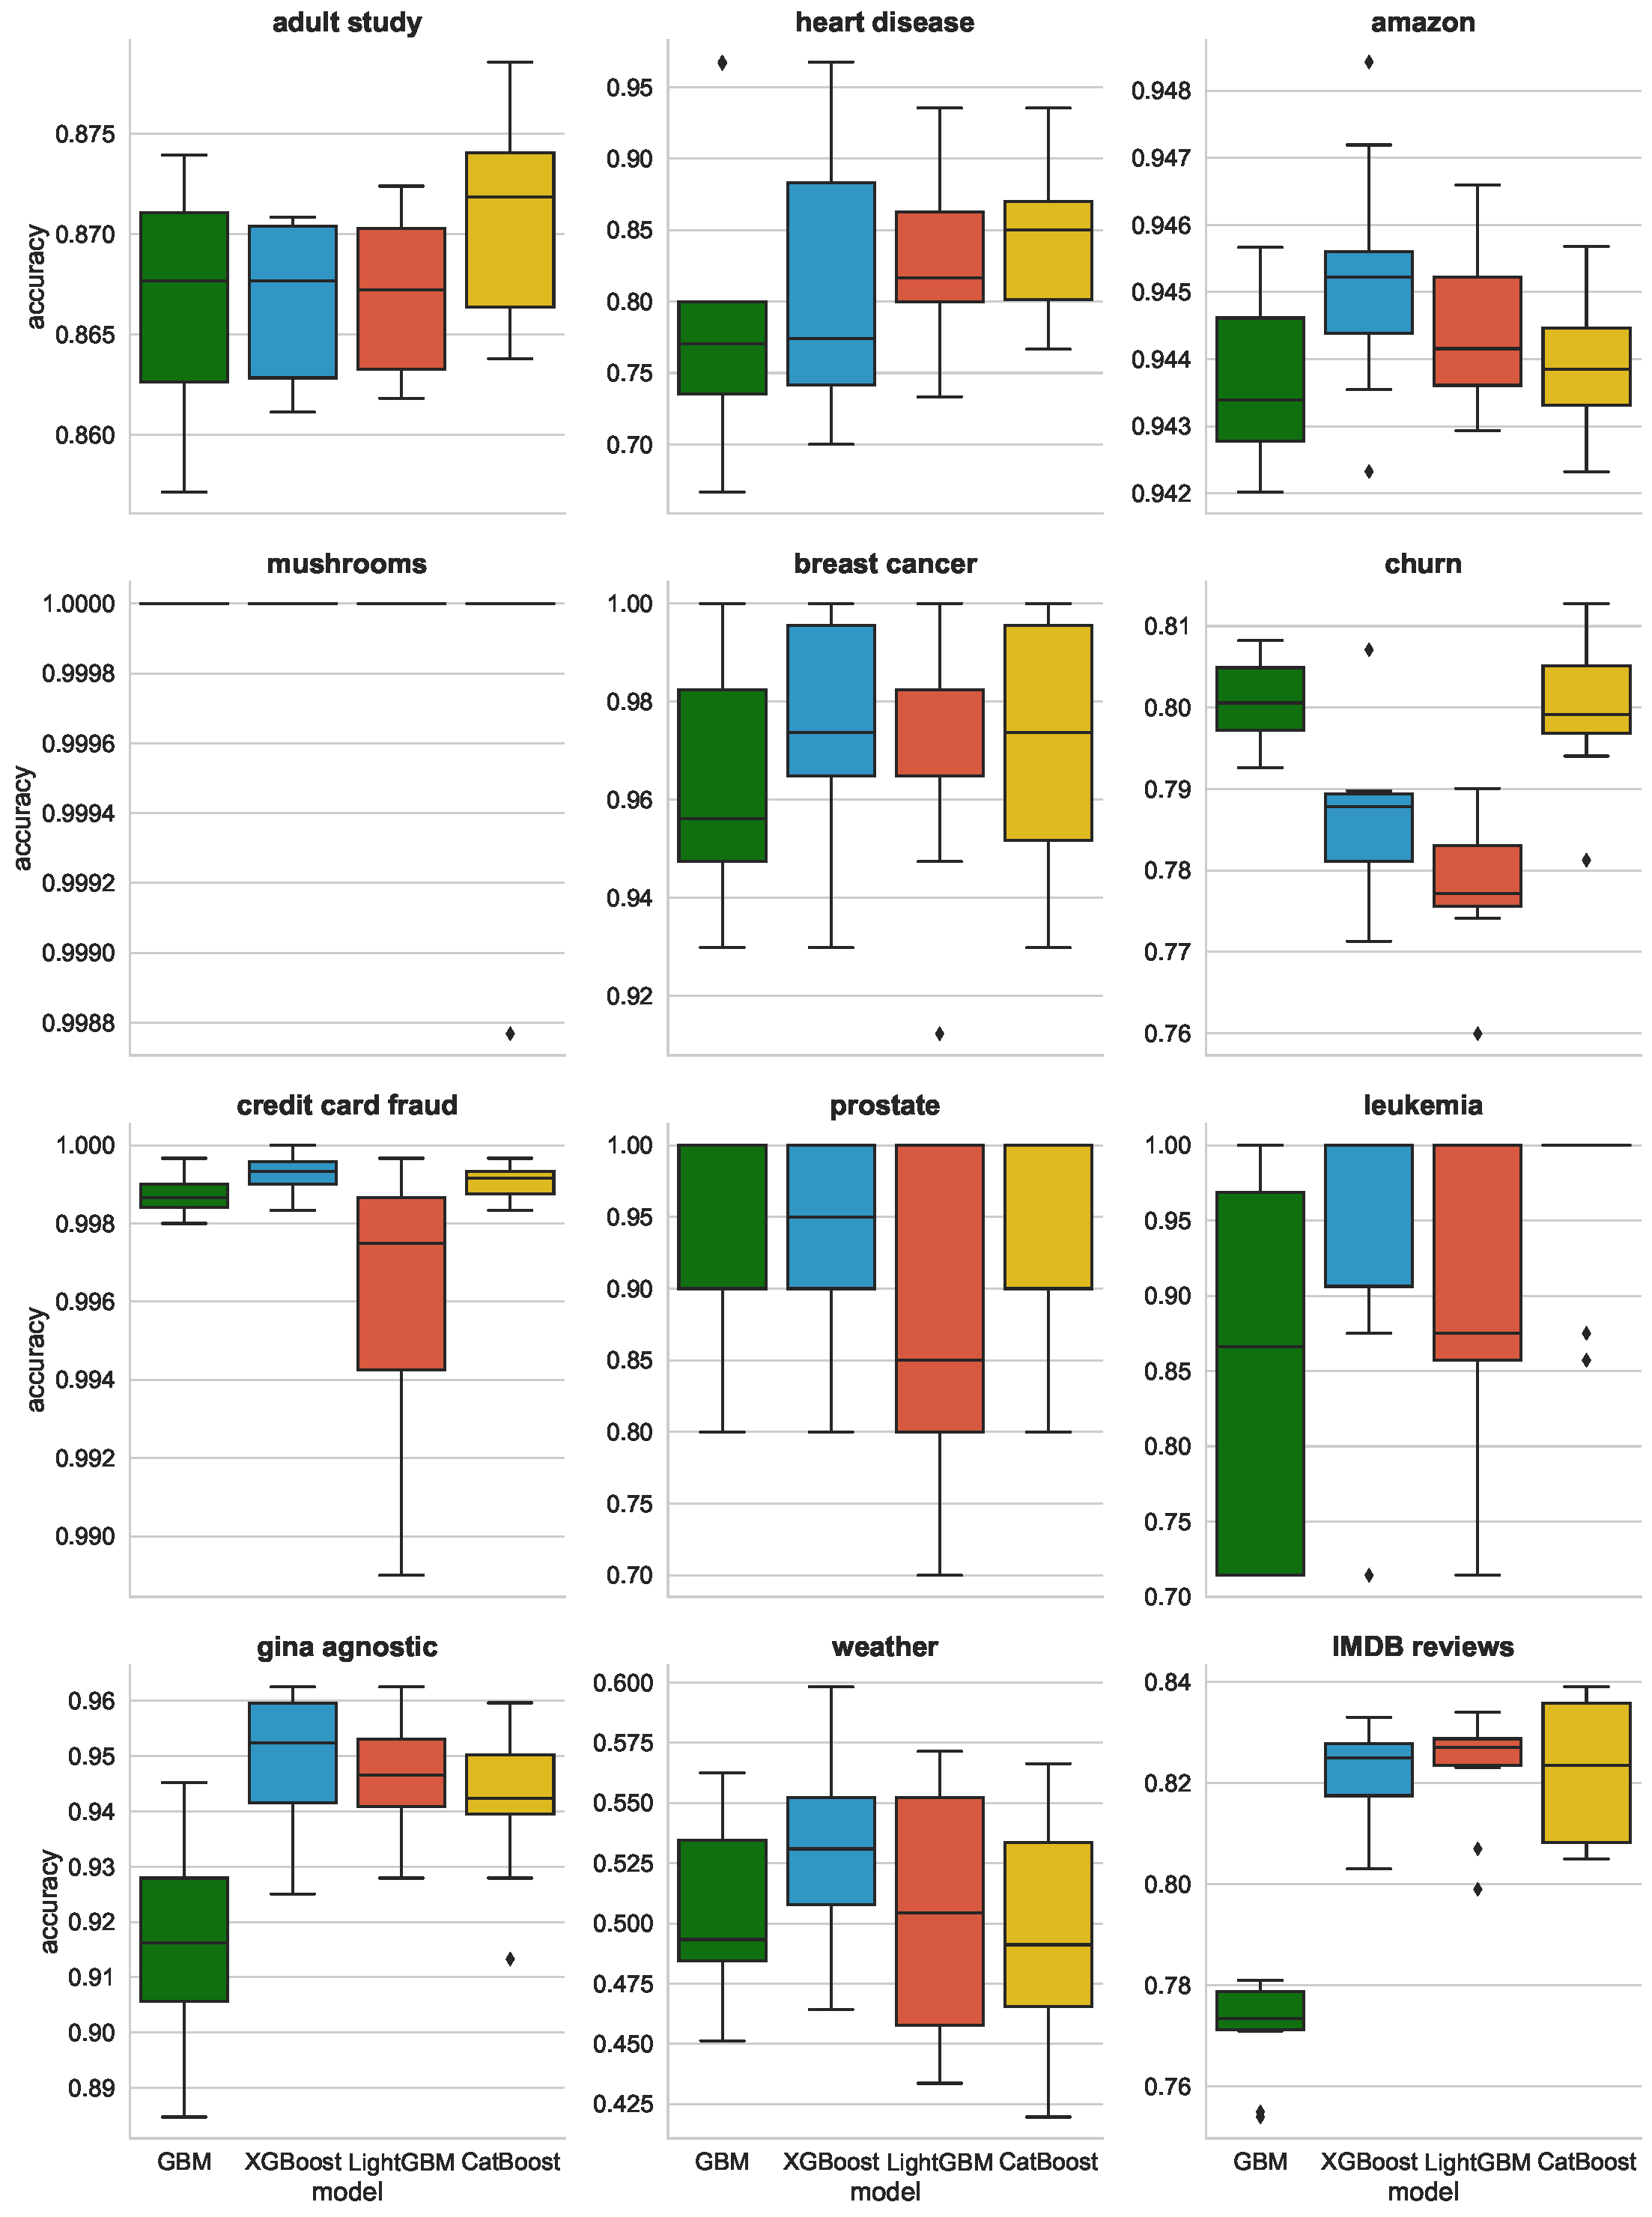
\includegraphics{plots/results_accuracy_12_datasets_no_tuning_150_50_trees_facet.pdf}}
	\caption{Accuracy distributions across 12 datasets without hyperparameter tuning}
	\label{fig:no_tuning_accuracy}
\end{figure}

Performance of each of the GBM implementation varies a lot when considering different datasets. There is no algorithm which would perform the best across all datasets, however, it can be observed that GBM proposed by Friedman \cite{friedman_gbm} almost always performs the worst (except for \emph{churn} and \emph{credit card fraud} datasets). Baseline versions of XGBoost and CatBoost seem to perform the best in terms of accuracy. 

Distributions presented in each of the boxplots can be characterized by their mean, standard devation or other statistics --- a summary has been presented in Table~\ref{tab:no_tuning_accuracy}.

\begin{table}[h!]
\centering
\begin{tabular}{|c|c|c|c|c|}
\hline
\textbf{dataset}  & \textbf{GBM}  & \textbf{XGBoost}  & \textbf{LightGBM}  & \textbf{CatBoost} \\ \hline
adult study & \cellcolor{red}0.867 $\pm$ 0.005 & 0.867 $\pm$ 0.004 & 0.867 $\pm$ 0.004 & \cellcolor{green}0.871 $\pm$ 0.005\\ \hline
heart disease &\cellcolor{red} 0.792 $\pm$ 0.101 & 0.808 $\pm$ 0.088 & 0.828 $\pm$ 0.061 & \cellcolor{green}0.841 $\pm$ 0.056\\ \hline
amazon & \cellcolor{red}0.944 $\pm$ 0.001 & \cellcolor{green}0.945 $\pm$ 0.002 & \cellcolor{red}0.944 $\pm$ 0.001 & \cellcolor{red}0.944 $\pm$ 0.001\\ \hline
mushrooms & 1.0 $\pm$ 0.0 & 1.0 $\pm$ 0.0 & 1.0 $\pm$ 0.0 & 1.0 $\pm$ 0.0\\ \hline
breast cancer & \cellcolor{red}0.963 $\pm$ 0.023 & \cellcolor{green}0.974 $\pm$ 0.024 & 0.967 $\pm$ 0.024 & 0.97 $\pm$ 0.027\\ \hline
churn & \cellcolor{green}0.801 $\pm$ 0.005 & 0.786 $\pm$ 0.01 & \cellcolor{red}0.778 $\pm$ 0.008 & 0.8 $\pm$ 0.009\\ \hline
credit card fraud & 0.999 $\pm$ 0.001 & \cellcolor{green}0.999 $\pm$ 0.0 & \cellcolor{red}0.996 $\pm$ 0.003 & \cellcolor{green}0.999 $\pm$ 0.0\\ \hline
prostate & 0.92 $\pm$ 0.079 & 0.94 $\pm$ 0.07 & \cellcolor{red}0.88 $\pm$ 0.114 & \cellcolor{green}0.95 $\pm$ 0.071\\ \hline
leukemia & \cellcolor{red}0.846 $\pm$ 0.126 & 0.946 $\pm$ 0.097 & 0.904 $\pm$ 0.095 & \cellcolor{green}0.973 $\pm$ 0.057\\ \hline
gina agnostic & \cellcolor{red}0.917 $\pm$ 0.019 & \cellcolor{green}0.949 $\pm$ 0.013 & 0.947 $\pm$ 0.01 & 0.941 $\pm$ 0.013\\ \hline
weather & 0.505 $\pm$ 0.038 & \cellcolor{green}0.53 $\pm$ 0.04 & 0.504 $\pm$ 0.052 & \cellcolor{red}0.495 $\pm$ 0.047\\ \hline
IMDB reviews & \cellcolor{red}0.772 $\pm$ 0.01 & 0.822 $\pm$ 0.01 & \cellcolor{green}0.823 $\pm$ 0.011 & 0.822 $\pm$ 0.014\\ \hline
\end{tabular}
\caption{Means and standard deviations of accuracy distributions presented in Figure~\ref{fig:no_tuning_accuracy}}
\label{tab:no_tuning_accuracy}
\end{table}

For each dataset, the best performing models have been marked with green color while the worst ones have been marked with red. Values of mean and standard deviation presented in Table~\ref{tab:no_tuning_accuracy} suggest that indeed baseline versions of XGBoost and CatBoost perform the best --- authors of corresponding implementations \cite{xgboost}, \cite{catboost} most likely put a lot of effort into choosing the best combination of default hyperparameters. On the other hand, GBM and LightGBM tend to perform the worst; for both of them, in some cases the standard deviations of accuracy are quite big, which indicate that baseline versions of GBM and LightGBM do not generalize as well as XGBoost and CatBoost. There are two possible causes which can explain the instability of the results: firstly, GBM lacks L1 and L2 regularization and in the case of LightGBM, values of aforementioned regularization are set to zero by default. For XGBoost and CatBoost, the default value of $\lambda$ used in L2 regularization has been set to 1 and 3, respectively. Secondly, LightGBM uses leaf-wise growth by default, which may lead to overfitting in situation where other hyperparameters are not taken into consideration\footnote{The explanation is provided in LightGBM's documentation: \url{lightgbm.readthedocs.io/en/latest/Parameters-Tuning.html}}.  

Similar conclusions can be drawn while analyzing classifiers' performance in terms of F1 score instead of accuracy. However, since AUC takes evaluates models' performance in a different way than accuracy and F1 score, obtained results are quite different --- they have been presented in Figure~\ref{fig:no_tuning_AUC}. 
 
\iffalse
\begin{figure}[H]
	\centering
		\scalebox{0.42}{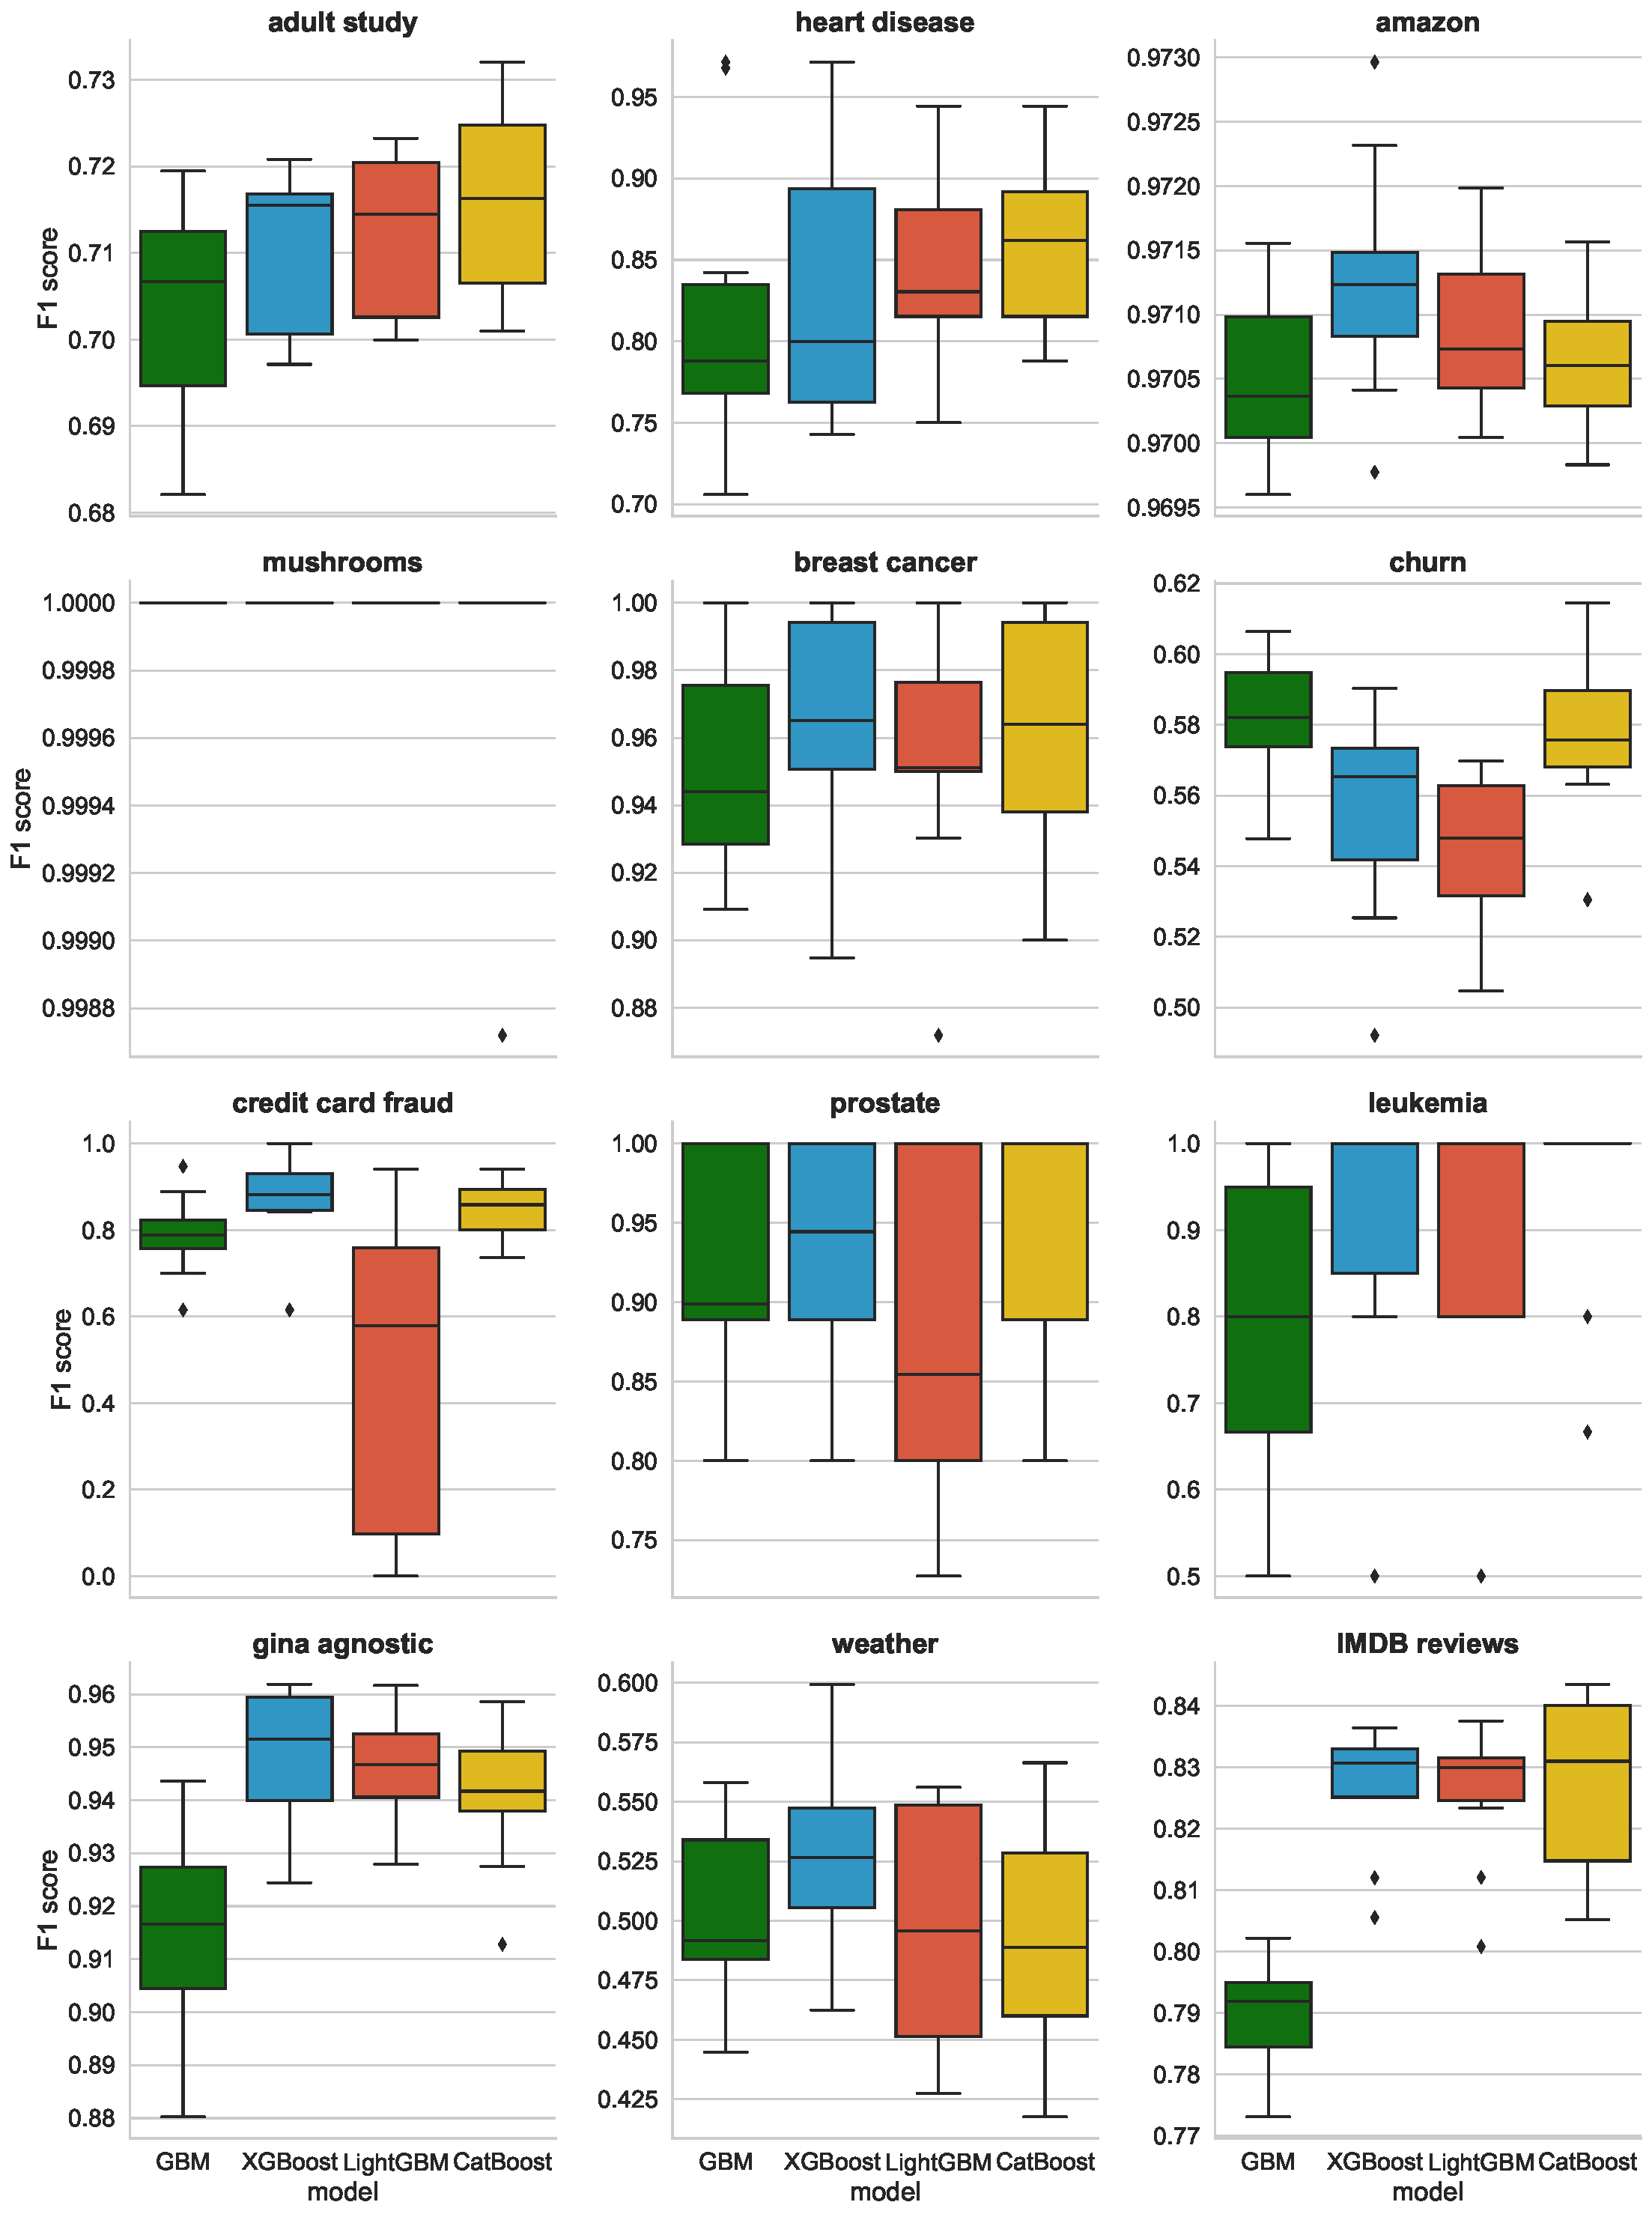
\includegraphics{main/plots/results_f1_score_12_datasets_no_tuning_150_50_trees_facet.pdf}}
	\caption{F1 score distributions across 12 datasets without hyperparameter tuning}
	\label{fig:no_tuning_F1}
\end{figure}
\fi

\begin{figure}[H]
	\centering
		\scalebox{0.42}{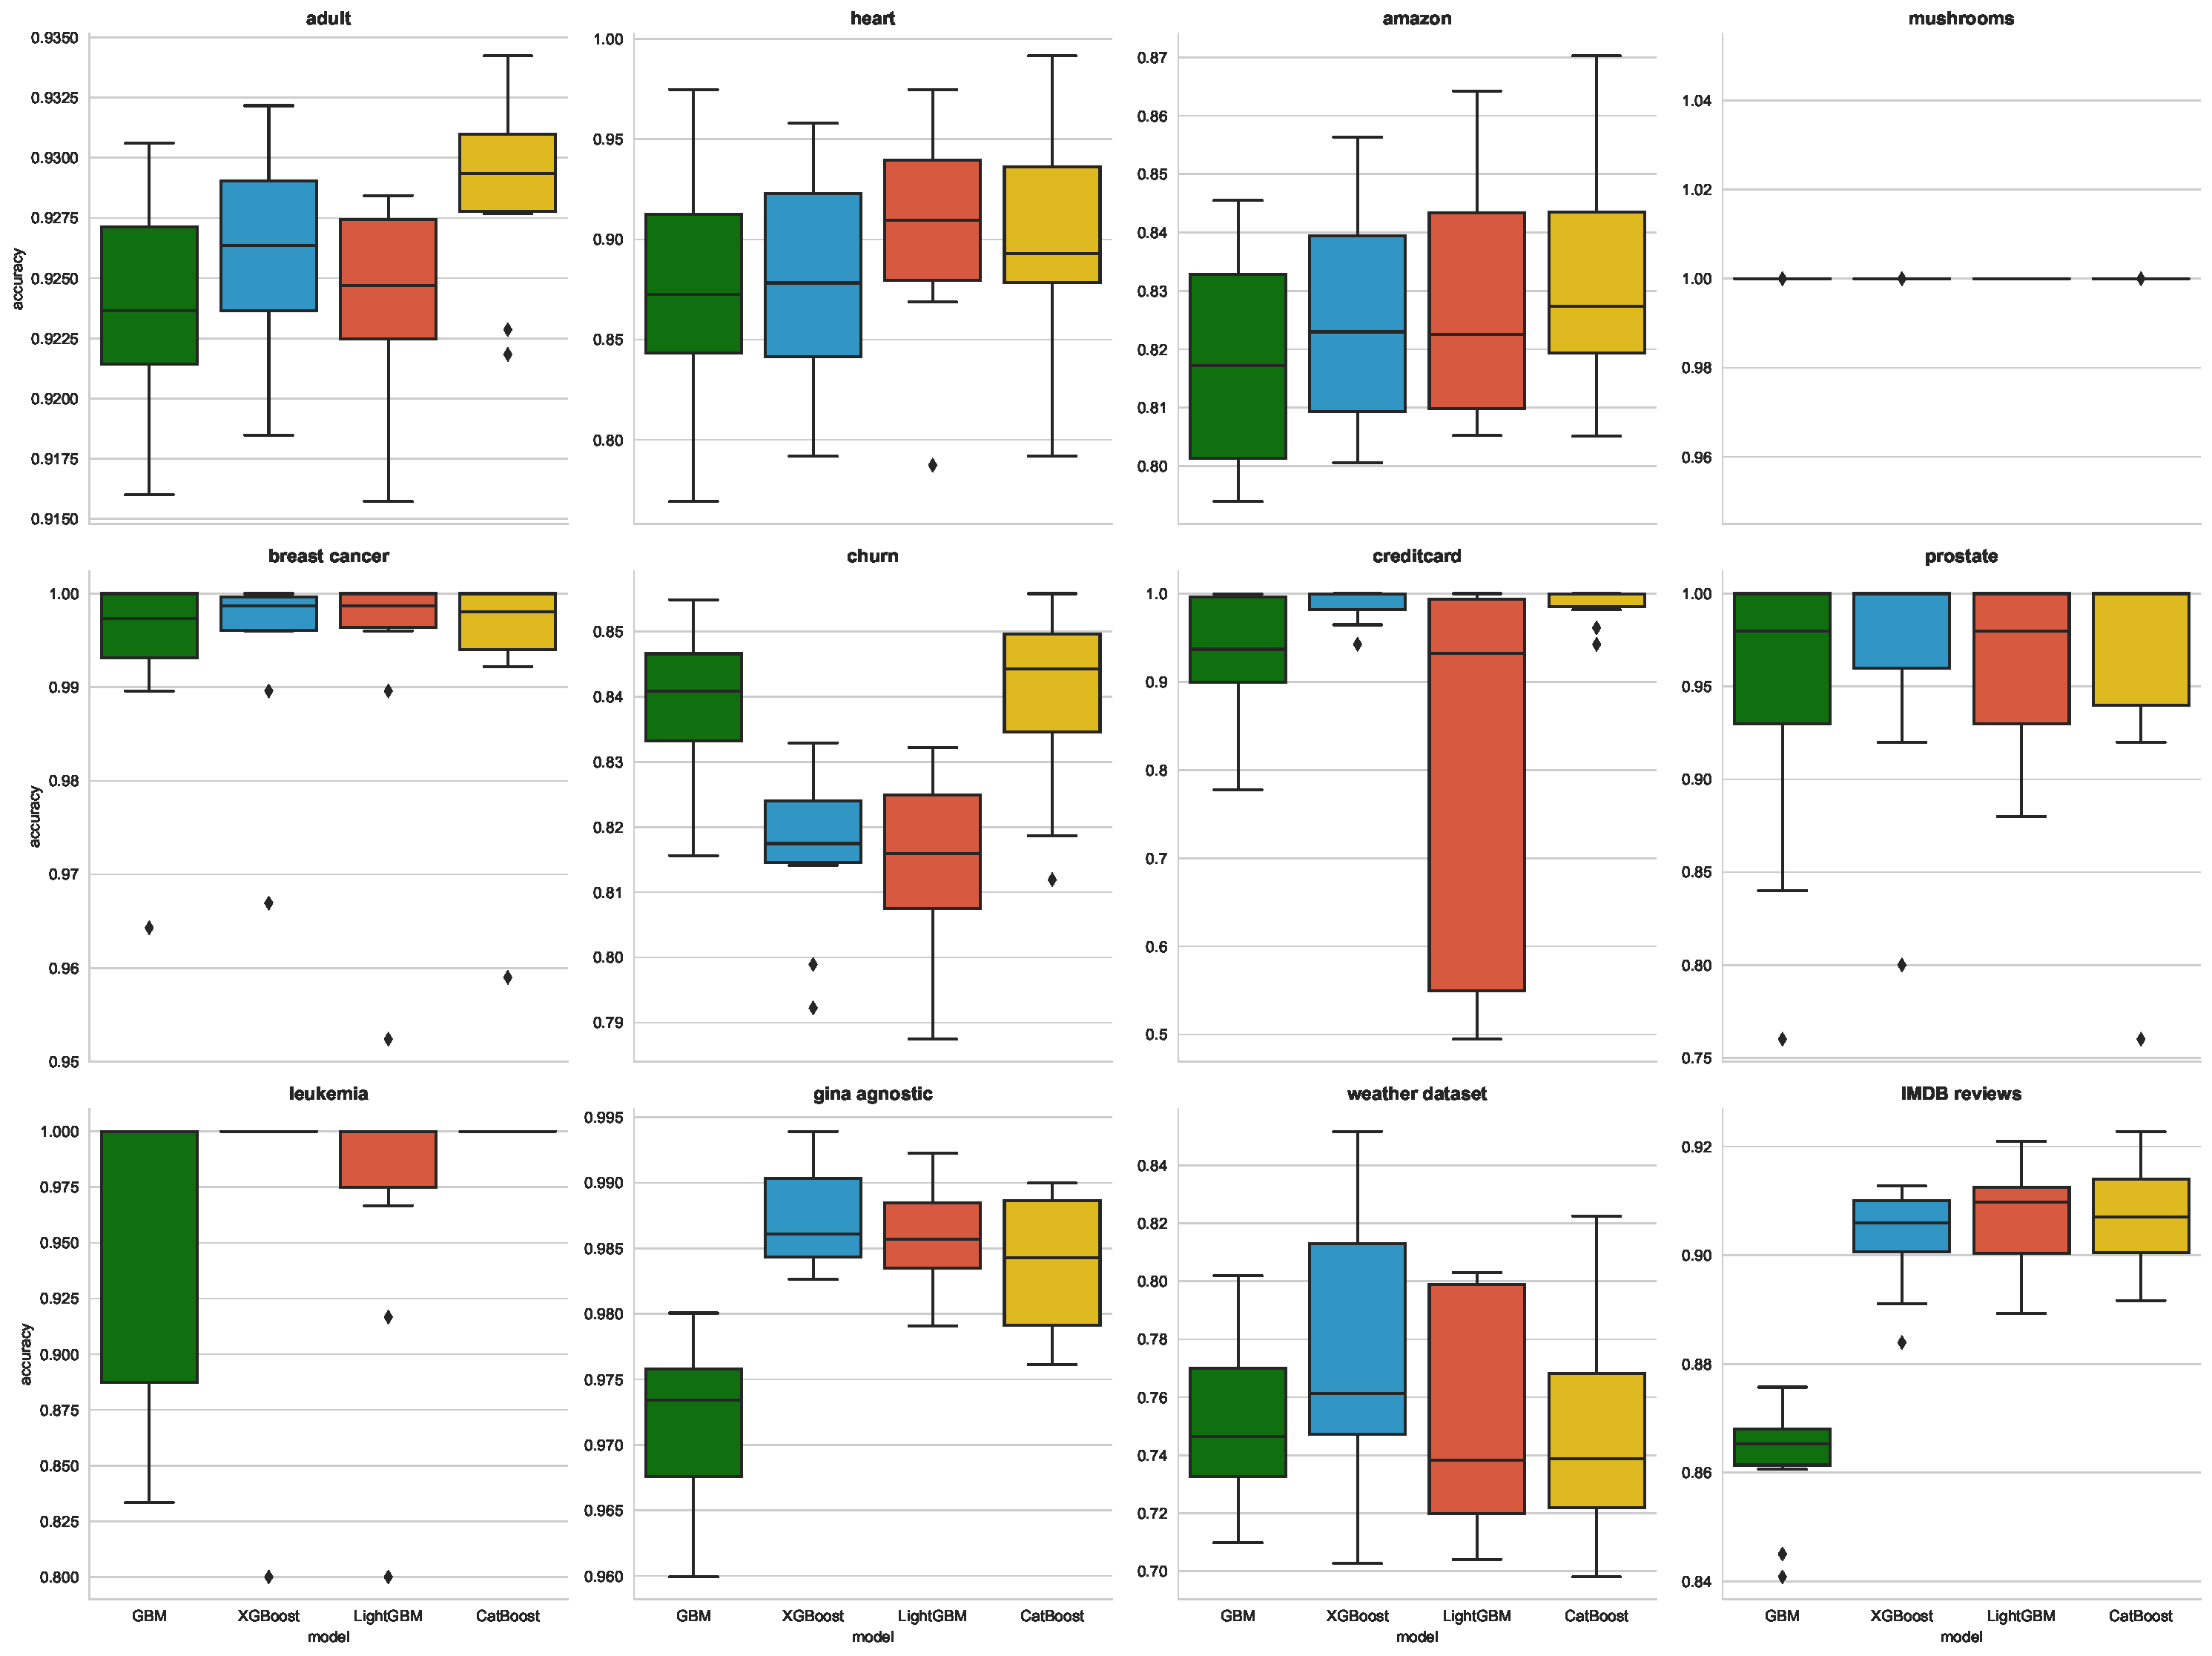
\includegraphics{main/plots/results_AUC_12_datasets_no_tuning_150_50_trees_facet.pdf}}
	\caption{AUC distributions across 12 datasets without hyperparameter tuning}
	\label{fig:no_tuning_AUC}
\end{figure}

In Figure~\ref{fig:no_tuning_AUC} an enormous degradation in terms of AUC in case of LightGBM and the \emph{credit card fraud} dataset can be seen almost immediately. While accuracy (Figure~\ref{fig:no_tuning_accuracy}) ranged from 0.994 to around 0.998, AUC can be as low as 0.55 --- this behaviour is concerning. On the other hand, AUC seem to vary a lot less compared to accuracy in case of \emph{leukemia} and \emph{prostate} datasets. Numerical summary of AUC scores have been presented in Table~\ref{tab:no_tuning_AUC}.

\begin{table}[h!]
\centering
\begin{tabular}{|c|c|c|c|c|}
\hline
\textbf{dataset}  & \textbf{GBM}  & \textbf{XGBoost}  & \textbf{LightGBM}  & \textbf{CatBoost} \\ \hline
adult study & \cellcolor{red}0.924 $\pm$ 0.005 & 0.926 $\pm$ 0.004 & \cellcolor{red}0.924 $\pm$ 0.005 & \cellcolor{green}0.929 $\pm$ 0.004\\ \hline
heart disease & \cellcolor{red}0.875 $\pm$ 0.064 & 0.878 $\pm$ 0.056 & \cellcolor{green}0.904 $\pm$ 0.053 & 0.9 $\pm$ 0.056\\ \hline
amazon & \cellcolor{red}0.819 $\pm$ 0.019 & 0.825 $\pm$ 0.019 & 0.828 $\pm$ 0.021 & \cellcolor{green}0.832 $\pm$ 0.021\\ \hline
mushrooms & 1.0 $\pm$ 0.0 & 1.0 $\pm$ 0.0 & 1.0 $\pm$ 0.0 & 1.0 $\pm$ 0.0\\ \hline
breast cancer & 0.994 $\pm$ 0.011 & \cellcolor{green}0.994 $\pm$ 0.01 & \cellcolor{red}0.993 $\pm$ 0.015 & 0.994 $\pm$ 0.013\\ \hline
churn & 0.839 $\pm$ 0.012 & 0.817 $\pm$ 0.013 & \cellcolor{red}0.814 $\pm$ 0.014 & \cellcolor{green}0.84 $\pm$ 0.014\\ \hline
credit card fraud & 0.933 $\pm$ 0.071 & \cellcolor{green}0.988 $\pm$ 0.02 & \cellcolor{red}0.803 $\pm$ 0.229 & \cellcolor{green}0.988 $\pm$ 0.02\\ \hline
prostate & \cellcolor{red}0.944 $\pm$ 0.083 & 0.964 $\pm$ 0.064 & \cellcolor{green}0.964 $\pm$ 0.044 & 0.96 $\pm$ 0.078\\ \hline
leukemia & \cellcolor{red}0.952 $\pm$ 0.078 & 0.98 $\pm$ 0.063 & 0.968 $\pm$ 0.065 & \cellcolor{green}1.0 $\pm$ 0.0\\ \hline
gina agnostic & \cellcolor{red}0.972 $\pm$ 0.006 & \cellcolor{green}0.987 $\pm$ 0.004 & 0.986 $\pm$ 0.004 & 0.984 $\pm$ 0.005\\ \hline
weather & 0.751 $\pm$ 0.031 & \cellcolor{green}0.775 $\pm$ 0.046 & 0.753 $\pm$ 0.041 & \cellcolor{red}0.748 $\pm$ 0.039\\ \hline
IMDB reviews & \cellcolor{red}0.862 $\pm$ 0.011 & 0.903 $\pm$ 0.009 & \cellcolor{green}0.907 $\pm$ 0.01 & \cellcolor{green}0.907 $\pm$ 0.01\\ \hline
\end{tabular}
\caption{Means and standard deviations of AUC distributions presented in Figure~\ref{fig:no_tuning_AUC}}
\label{tab:no_tuning_AUC}
\end{table}

Holistically, AUC values across most of the datasets are higher than accuracy. In the case of the \emph{weather} dataset AUC values are higher than accuracy by around 50\%. Also, AUC values seem to have less spread out which is indicated by low values of standard deviations, however one has to keep in mind that AUC and accuracy scores cannot be compared directly. What is really interesting is that CatBoost has managed to achieve perfect AUC score on the \emph{leukemia} dataset. Overall, among baseline versions of GBM, XGBoost, LightGBM and CatBoost both XGBoost and CatBoost seem to perform the best it terms of accuracy, F1 score and AUC while GBM's performance is the worst.

On the other hand, accuracy, F1 score and AUC are not the only criteria which are used in this comparative analysis, the runtimes of the algorithms are also crucial --- in case of non-tuned models, times needed to perform model evaluation have been presented in Figure~\ref{fig:no_tuning_runtimes}.

\begin{figure}[H]
	\centering
		\scalebox{0.42}{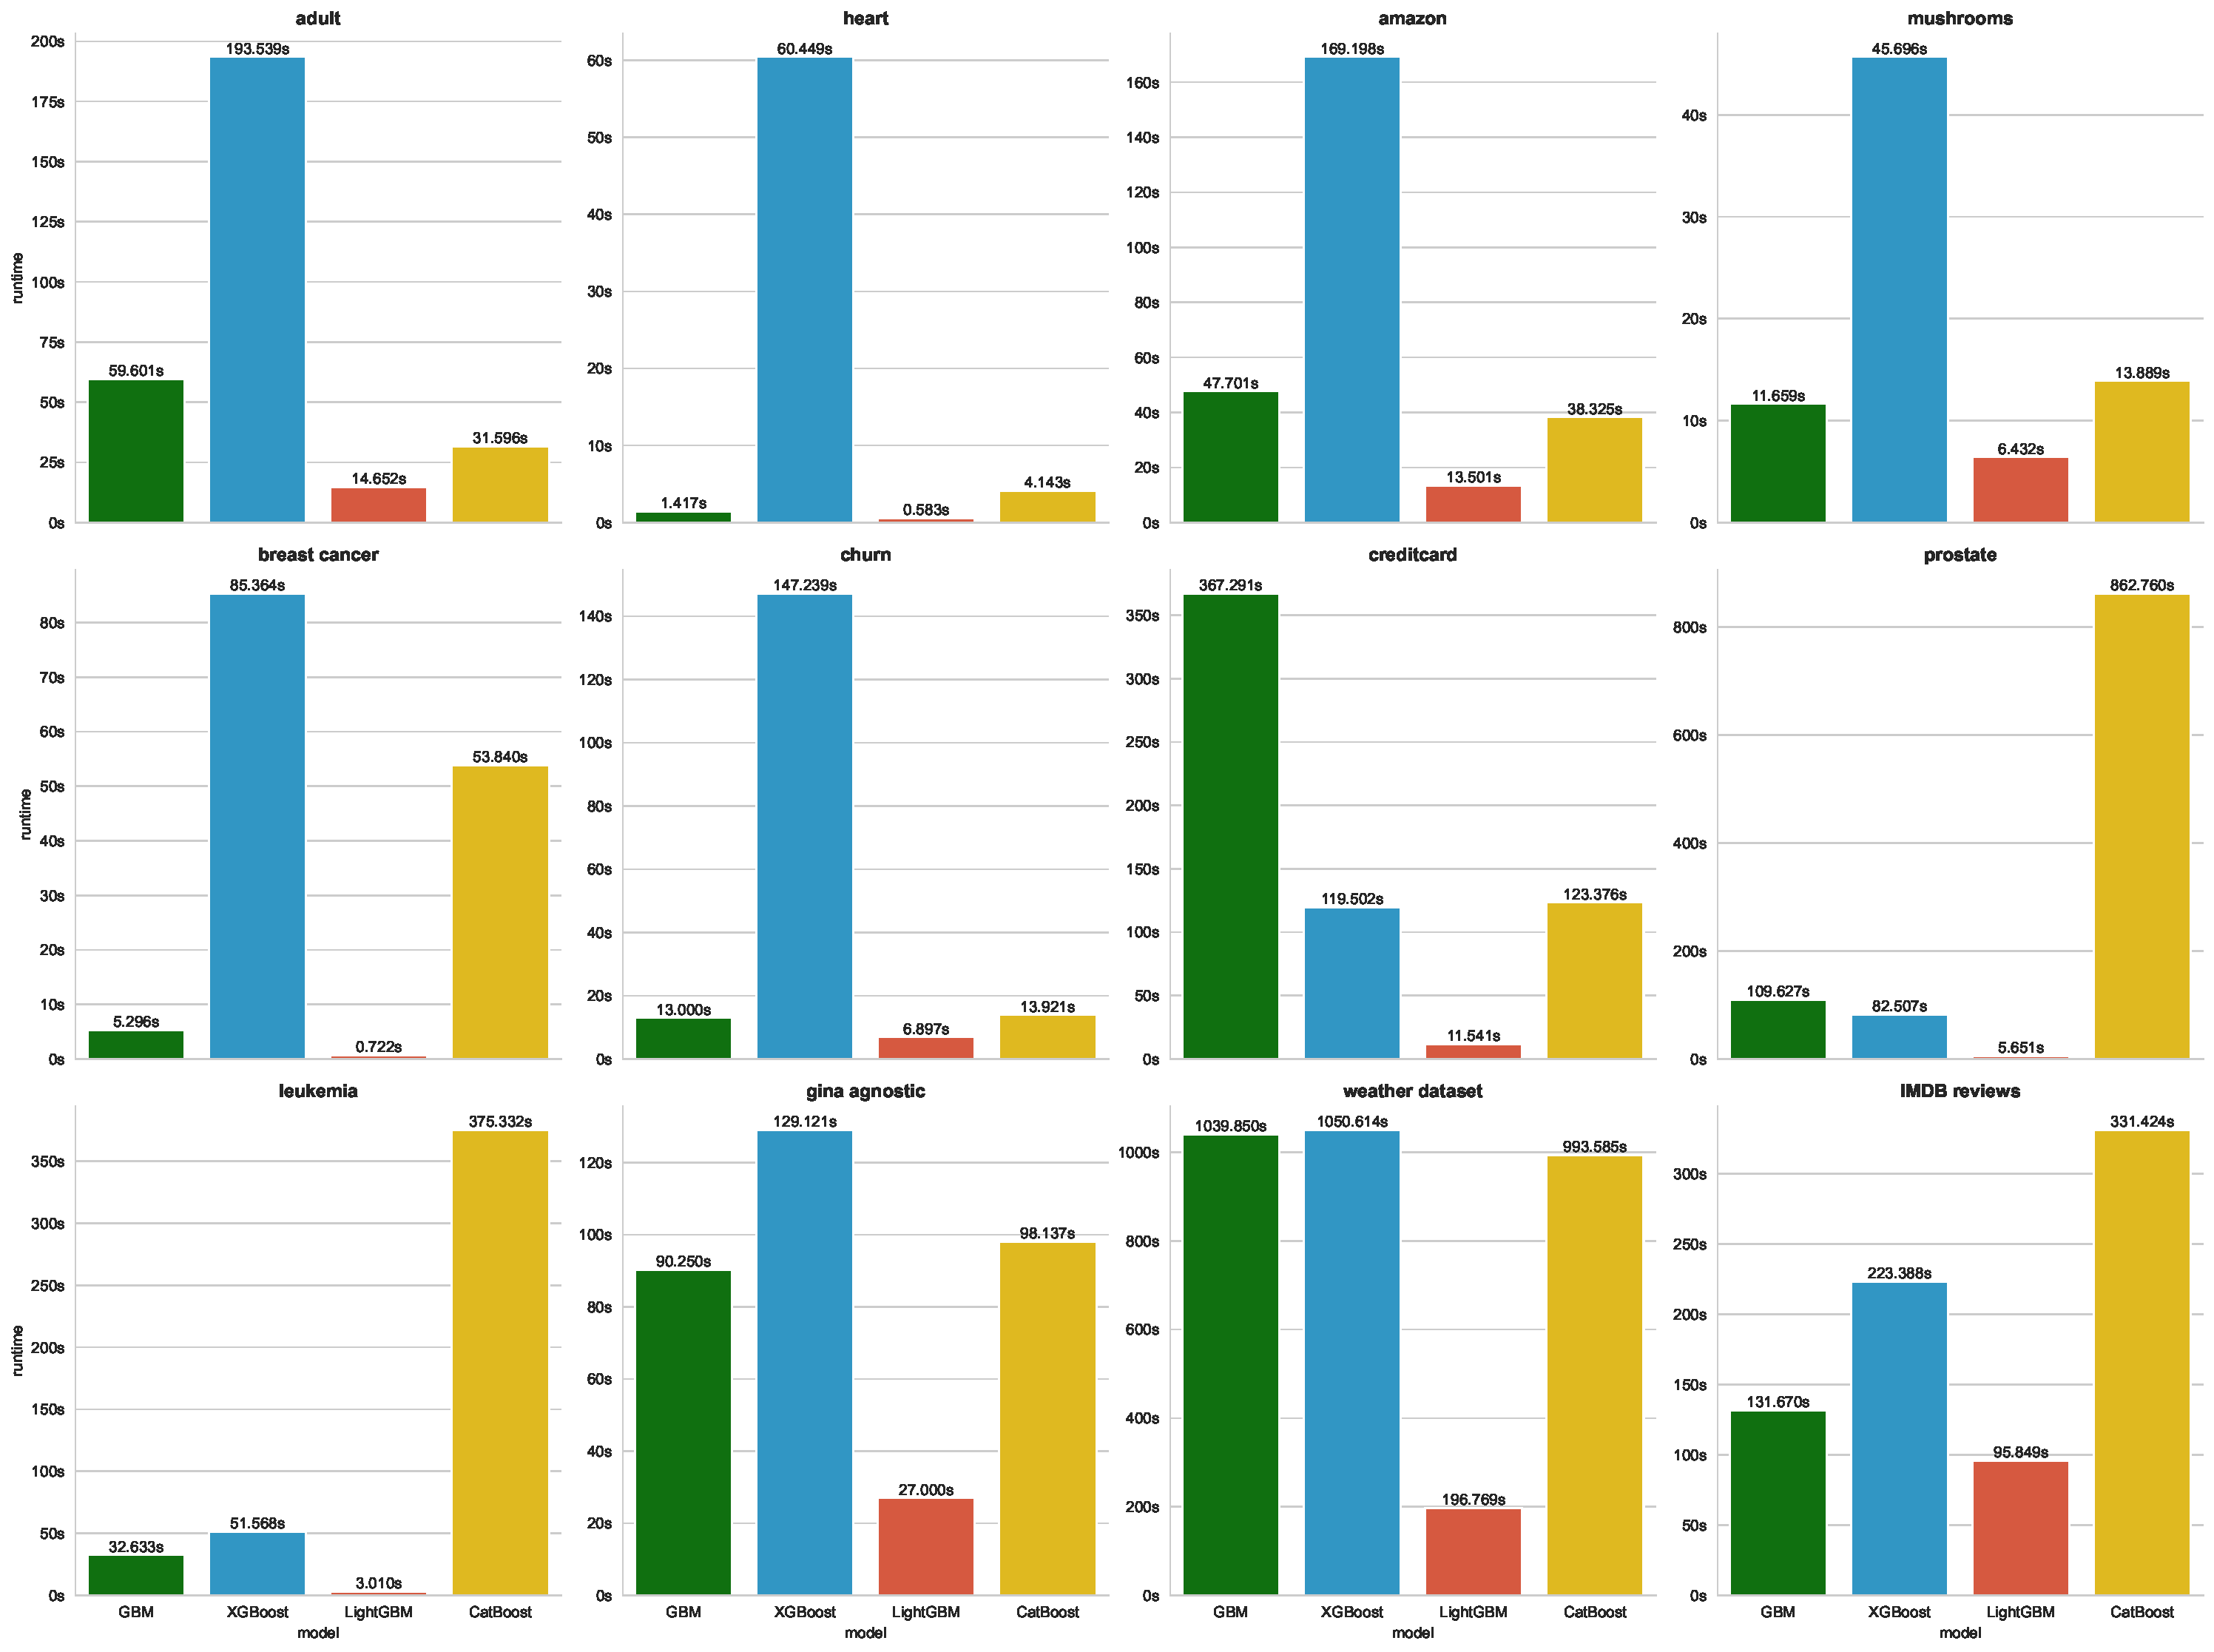
\includegraphics{main/plots/runtimes_12_datasets_no_tuning_150_50_trees_facet.pdf}}
	\caption{Runtimes of the models across 12 datasets without hyperparameter tuning}
	\label{fig:no_tuning_runtimes}
\end{figure}

Overall, the runtimes between models tend to vary a lot less than values of accuracy, F1 score or AUC. However, the models with the best evaluation metrics, namely XGBoost and CatBoost tend to be slower than GBM and much slower than LightGBM. In the case of the first six datasets presented in Table~\ref{tab:datasets}: \emph{adult study}, \emph{heart disease}, \emph{amazon}, \emph{mushrooms}, \emph{breast cancer} and \emph{churn} XGBoost is clearly the slowest. Aforementioned datasets vary greatly in the number of samples (\emph{adult study} has 48842 while \emph{heart disease} contains information about 303 instances), so the length of the datasets clearly had no impact on XGBoost's performance. Additionally, they contain a reasonable number of features (30 at most), so the exact splitting algorithm implemented in XGBoost should still work quite efficiently (even in the case of very highly dimensional data, namely \emph{prostate} and \emph{leukemia} it did well). Thus, the reason behind enormous runtimes of XGBoost on first six datasets presented in Table~\ref{tab:datasets} cannot be pointed out. 

On the other hand, except for one case (\emph{credit card fraud}) GBM tends to perform rather quickly depsite not being computationally optimized like state-of-the-art implementations. LightGBM is consistently the fastest algorithm across all datasets --- histogram-based splitting algorithm, GOSS, EFB and leaf-wise tree growth all greatly contribute to the greatly decreased runtime. Sometimes, LightGBM is faster than other GBM implementations even by up to two orders of magnitude. It scales very well with high number of samples and very high number of features. 

CatBoost's greatest strength lies in datasets with low to moderate number of features (an area where XGBoost surprisingly struggles). Great performance in terms of accuracy, F1 score and AUC can be achieved in a very competitive and reasonable amount of time (even despite using Ordered algorithm which is slower than the Plain one). CatBoost scales well with the number of instances, however, it completely cannot handle highly dimensional data. Plain version is much slower than other GBM implementations in case of \emph{prostate} and \emph{leukemia} datasets. In case of \emph{gina agnostic} dataset, it is slightly slower than GBM and noticeably faster than XGBoost. In the case of \emph{weather} dataset, Plain CatBoost is almost as slow as XGBoost and CatBoost. Excessive runtimes of CatBoost are surprising, because by default, the value of $\lambda$ responsible for L2 regularization is equal to 3 (to recall, $\lambda=1$ and $\lambda=0$ for XGBoost and LightGBM, respectively).

It has been observed that both Ordered and Plain CatBoost struggle with memory consumption when being used with highly dimensional datasets. Originally, the \emph{weather} dataset contained 4800 features, but Plain CatBoost could not handle that amount of data --- over 17GB of RAM was used, which is quite inefficient (other GBM implementations consumed less than 6GB of RAM). Thus, the size of \emph{weather} dataset had to be reduced to 2500. Such computational infeasibility of CatBoost in unacceptable, especially that it cannot be used with highly dimensional datasets on reasonably new personal computers or laptops (most of them will have up to 16GB of RAM memory). 

Friedman test with Nemenyi Post Hoc Analysis has been performed to rank the performance of non-tuned versions of \gbm across twelve datasets described in Table~\ref{tab:datasets}. The results in form of a heatmap have been presented in Figure~\ref{fig:no_tuning_accuracy_heatmap}. In each cell two values are displayed: the one in the upper left corner denotes the rank of the model on the left hand side of the side while the other one points at the rank of the model at the bottom.

\begin{figure}[H]
	\centering
		\scalebox{0.7}{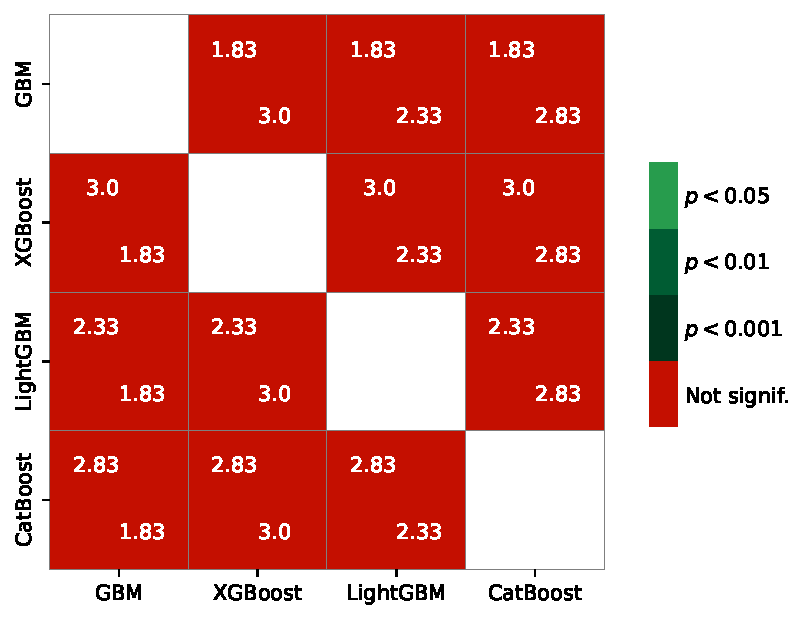
\includegraphics{main/plots/heatmap_accuracy_12_datasets_no_tuning_150_50_trees.pdf}}
	\caption{Ranking of models' accuracy scores. Critical difference $CD = 1.354$}
	\label{fig:no_tuning_accuracy_heatmap}
\end{figure}

The ranking could indicate that XGBoost is the most accurate baseline model. CatBoost's performance is similar, LightGBM and GBM are significantly worse. However, it cannot be explicitly stated that for example XGBoost is a better model than GBM, because the difference in ranks is lower than the Critical difference threshold equal to 1.354. Fortunately, in case of the F1 score XGboost is in fact better than GBM --- an illustration of the ranking have been presented in Figure~\ref{fig:no_tuning_F1_heatmap}.

\begin{figure}[H]
	\centering
		\scalebox{0.7}{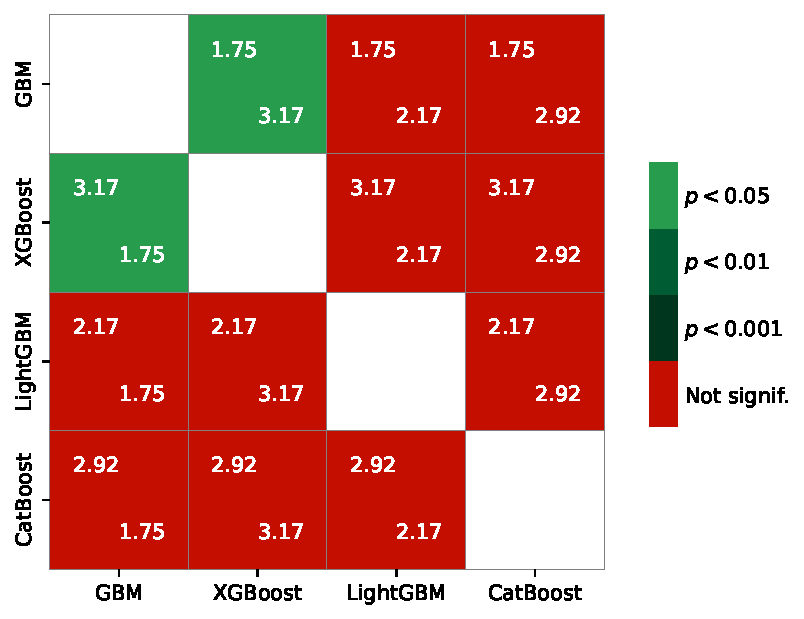
\includegraphics{main/plots/heatmap_f1_score_12_datasets_no_tuning_150_50_trees.pdf}}
	\caption{Ranking of models' F1 scores. Critical difference $CD = 1.354$}
	\label{fig:no_tuning_F1_heatmap}
\end{figure}

In case of F1 score the different of performance between GBM and XGBoost is bigger; it is also statistically significant. A similar observation can be made in case of AUC score. Final ranking of baseline variants of \gbm in terms of F1 score is as follows:

\begin{enumerate}
    \item XGBoost with rank 3.17
    \item CatBoost with rank 2.92
    \item LightGBM with rank 2.17
    \item GBM with rank 1.75
\end{enumerate}

\subsection{Analysis of models tuned with bayesian optimization}\label{section_tpe}
In this section, comparative analysis of \gbm models tuned using Tree Parzen Estimators have been carried out. The procedure which has been used for selection of optimal hyperparameters and evaluation of models have been described in Scheme~\ref{eval_scheme}. Due to the sequential nature of bayesian optimization, the number of tuning iterations for each of the gradient boosting implementation has been set to 15 (by default, only 10 iterations are performed). 

One of the aims of model selection in form of hyperparameter tuning is to find models with the best performance possible. Thus, it is absolutely essential to define a set of initial hyperparameters (further referred as \emph{init}) and a search space which will be used in the tuning. To preserve consistency with the experiment described in Section\ref{section:baseline}, the number of trees and \emph{boosting\_type} in case of LightGBM and CatBoost remain unchanged. Following the advice given in \cite{comparative_analysis} and in \cite{friedman_gbm}, the number of trees has been fixed to the highest computationally feasible value (to recall, it is equal to 150 except for \emph{gina agnostic}, \emph{weather} and \emph{IMDB reviews} datasets where it has been set to 50) and consequently \emph{learning\_rate} will be one of the tuned hyperparameters.

In case of other hyperparameters used in \emph{init} and tuning, an extensive study of each of the GBM implementations' documentation has been carried out. Documentations greatly vary in lengths: gradient boosting\footnote{\url{scikit-learn.org/stable/modules/generated/sklearn.ensemble.GradientBoostingClassifier}} has the shortest one, followed by CatBoost\footnote{\url{catboost.ai/en/docs/references/training-parameters/}}; XGBoost\footnote{\url{xgboost.readthedocs.io/en/stable/parameter.html}} and LightGBM\footnote{\url{lightgbm.readthedocs.io/en/latest/Parameters.html}} in particular provide the most exhaustive documentations, because their implementations \cite{xgboost}, \cite{lightgbm} contain the biggest number of available hyperparameters. Additionally, Friedman's advice regarding stochastic gradient boosting \cite{friedman_stoch} has been considered, as well as the choice of hyperparameters and search spaces which were described in \cite{catboost}, \cite{comparative_analysis} and \cite{competitive_analysis}. The conclusions from the studied documentations and literature suggest the following:
\begin{enumerate}
    \item As it has been stated before, the number of trees has been fixed, but \emph{learning\_rate} is tuned
    \item In conjunction with the advice given in \cite{friedman_stoch} and \cite{comparative_analysis}, instances and features subsampling have been set to fixed values; it is not worth to tune them
    \item In \cite{catboost}, \cite{comparative_analysis} and \cite{competitive_analysis} the maximum depth of a tree (or number of leaves in case of LightGBM), L1 and L2 regularization were common hyperparameters which were tuned, so in this work they will also be a part of the search spaces
    \item Also, algorithm-specific hyperparameters are a common choice during the process of model selection, thus they will also be considered. These include: XGBoost's \emph{gamma}, LightGBM's \emph{top\_rate} and \emph{other\_rate} and CatBoost's \emph{leaf\_estimation\_iterations}. 
\end{enumerate}

Additionally, some \emph{init} hyperparameters as well as some search spaces are different in case of various datasets. For those with a small number of samples, \emph{subsample} has been set to 1 --- excessive subsampling of a dataset which is already small can lead to a degradation of performance. Moreover, upper bound of regularization strength in search spaces has been increased in datasets with very high number of features.

The summary of initial hyperparametrization as well as search spaces has been presented in Table~\ref{tab:init_tuning}. In search spaces, discrete values in square brackets are sampled uniformly, while continuous ones are sampled either from uniform ($\mathcal{U}$) or log-uniform ($\log\mathcal{U}$) distributions.

\begin{landscape}
\begin{table}[]
\centering
\resizebox{670pt}{!}{%
\begin{tabular}{ccccc}
\hline
\multicolumn{1}{|c|}{\textbf{datasets}} &
  \multicolumn{1}{c|}{\textbf{\begin{tabular}[c]{@{}c@{}}GBM\\ init\end{tabular}}} &
  \multicolumn{1}{c|}{\textbf{\begin{tabular}[c]{@{}c@{}}XGBoost\\ init\end{tabular}}} &
  \multicolumn{1}{c|}{\textbf{\begin{tabular}[c]{@{}c@{}}LightGBM\\ init\end{tabular}}} &
  \multicolumn{1}{c|}{\textbf{\begin{tabular}[c]{@{}c@{}}CatBoost\\ init\end{tabular}}} \\ \hline
\multicolumn{1}{|c|}{\begin{tabular}[c]{@{}c@{}}adult study\\ amazon\\ mushrooms\\ churn\\ credit card fraud\end{tabular}} &
  \multicolumn{1}{c|}{\begin{tabular}[c]{@{}c@{}}n\_estimators: 150\\ subsample: 0.75\\ max\_features: 0.6\end{tabular}} &
  \multicolumn{1}{c|}{\begin{tabular}[c]{@{}c@{}}n\_estimators: 150\\ subsample: 0.75\\ colsample\_bynode: 0.6\end{tabular}} &
  \multicolumn{1}{c|}{\begin{tabular}[c]{@{}c@{}}boosting\_type: "goss"\\ n\_estimators: 150\\ subsample: 0.75\\ colsample\_bynode: 0.6\end{tabular}} &
  \multicolumn{1}{c|}{\begin{tabular}[c]{@{}c@{}}boosting\_type: "Ordered"\\ n\_estimators: 150\\ subsample: 0.75\\ colsample\_bylevel: 0.6\end{tabular}} \\ \hline
\multicolumn{1}{|c|}{\begin{tabular}[c]{@{}c@{}}heart disease\\ breast cancer\end{tabular}} &
  \multicolumn{1}{c|}{\begin{tabular}[c]{@{}c@{}}Same as above,\\  but with subsample = 1\end{tabular}} &
  \multicolumn{1}{c|}{\begin{tabular}[c]{@{}c@{}}Same as above,\\  but with subsample = 1\end{tabular}} &
  \multicolumn{1}{c|}{\begin{tabular}[c]{@{}c@{}}Same as above,\\  but with subsample = 1\end{tabular}} &
  \multicolumn{1}{c|}{\begin{tabular}[c]{@{}c@{}}Same as above,\\  but with subsample = 1\end{tabular}} \\ \hline
\multicolumn{1}{|c|}{\begin{tabular}[c]{@{}c@{}}prostate\\ leukemia\end{tabular}} &
  \multicolumn{1}{c|}{\begin{tabular}[c]{@{}c@{}}n\_estimators: 150\\ subsample: 1\\ max\_features: 0.4\end{tabular}} &
  \multicolumn{1}{c|}{\begin{tabular}[c]{@{}c@{}}n\_estimators: 150\\ subsample: 1\\ colsample\_bynode: 0.4\end{tabular}} &
  \multicolumn{1}{c|}{\begin{tabular}[c]{@{}c@{}}boosting\_type: "goss"\\ n\_estimators: 150\\ subsample: 1\\ colsample\_bynode: 0.4\end{tabular}} &
  \multicolumn{1}{c|}{\begin{tabular}[c]{@{}c@{}}boosting\_type: "Plain"\\ n\_estimators: 150\\ subsample: 1\\ colsample\_bylevel: 0.4\end{tabular}} \\ \hline
\multicolumn{1}{|c|}{\begin{tabular}[c]{@{}c@{}}gina agnostic\\ weather\\ IMDB reviews\end{tabular}} &
  \multicolumn{1}{c|}{\begin{tabular}[c]{@{}c@{}}n\_estimators: 50\\ subsample: 0.5\\ max\_features: 0.4\end{tabular}} &
  \multicolumn{1}{c|}{\begin{tabular}[c]{@{}c@{}}n\_estimators: 50\\ subsample: 0.5\\ colsample\_bynode: 0.4\end{tabular}} &
  \multicolumn{1}{c|}{\begin{tabular}[c]{@{}c@{}}boosting\_type: "goss"\\ n\_estimators: 50\\ subsample: 0.5\\ colsample\_bynode: 0.4\end{tabular}} &
  \multicolumn{1}{c|}{\begin{tabular}[c]{@{}c@{}}boosting\_type: "Plain"\\ n\_estimators: 50\\ subsample: 0.5\\ colsample\_bylevel: 0.4\end{tabular}} \\ \hline
 &
   &
   &
   &
   \\ \hline
\multicolumn{1}{|c|}{\textbf{datasets}} &
  \multicolumn{1}{c|}{\textbf{\begin{tabular}[c]{@{}c@{}}GBM\\ tuning\end{tabular}}} &
  \multicolumn{1}{c|}{\textbf{\begin{tabular}[c]{@{}c@{}}XGBoost\\ tuning\end{tabular}}} &
  \multicolumn{1}{c|}{\textbf{\begin{tabular}[c]{@{}c@{}}LightGBM\\ tuning\end{tabular}}} &
  \multicolumn{1}{c|}{\textbf{\begin{tabular}[c]{@{}c@{}}CatBoost\\ tuning\end{tabular}}} \\ \hline
\multicolumn{1}{|c|}{\begin{tabular}[c]{@{}c@{}}adult study\\ amazon\\ mushrooms\\ churn\\ credit card fraud\end{tabular}} &
  \multicolumn{1}{c|}{\begin{tabular}[c]{@{}c@{}}max\_depth: [2, 3, 4, 5, 8, 10]\\ learning\_rate: \logU(0.01, 0.3)\\ min\_samples\_split: [2, 5, 10]\end{tabular}} &
  \multicolumn{1}{c|}{\begin{tabular}[c]{@{}c@{}}max\_depth: [2, 3, 4, 5, 8, 10]\\ learning\_rate: \logU(0.01, 0.3)\\ gamma: \U(0, 3)\\ alpha: \U(0, 1)\\ lambda: \U(0, 3)\end{tabular}} &
  \multicolumn{1}{c|}{\begin{tabular}[c]{@{}c@{}}num\_leaves: [3, 7, 15, 31, 127]\\ learning\_rate: \logU(0.01, 0.3)\\ top\_rate: \U(0.1, 0.5)\\ other\_rate: \U(0.05, 0.2)\\ reg\_alpha: \U(0, 1)\\ reg\_lambda: \U(0, 3)\end{tabular}} &
  \multicolumn{1}{c|}{\begin{tabular}[c]{@{}c@{}}max\_depth: [2, 3, 4, 5, 8, 10]\\ leaf\_estimation\_iterations: [1, 10]\\ l2\_leaf\_reg: \U(0, 5)\end{tabular}} \\ \hline
\multicolumn{1}{|c|}{\begin{tabular}[c]{@{}c@{}}heart disease\\ breast cancer\end{tabular}} &
  \multicolumn{1}{c|}{Same as above} &
  \multicolumn{1}{c|}{Same as above} &
  \multicolumn{1}{c|}{Same as above} &
  \multicolumn{1}{c|}{Same as above} \\ \hline
\multicolumn{1}{|c|}{\begin{tabular}[c]{@{}c@{}}prostate\\ leukemia\end{tabular}} &
  \multicolumn{1}{c|}{\begin{tabular}[c]{@{}c@{}}max\_depth: [2, 3, 4, 5, 8, 10]\\ learning\_rate: \logU(0.01, 0.3)\\ min\_samples\_split: [2, 5, 10]\end{tabular}} &
  \multicolumn{1}{c|}{\begin{tabular}[c]{@{}c@{}}max\_depth: [2, 3, 4, 5, 8, 10]\\ learning\_rate: \logU(0.01, 0.3)\\ gamma: \U(0, 10)\\ alpha: \U(0, 5)\\ lambda: \U(0, 10)\end{tabular}} &
  \multicolumn{1}{c|}{\begin{tabular}[c]{@{}c@{}}num\_leaves: [3, 7, 15, 31, 127]\\ learning\_rate: \logU(0.01, 0.3)\\ top\_rate: \U(0.1, 0.5)\\ other\_rate: \U(0.05, 0.2)\\ reg\_alpha: \U(0, 5)\\ reg\_lambda: \U(0, 10)\end{tabular}} &
  \multicolumn{1}{c|}{\begin{tabular}[c]{@{}c@{}}max\_depth: [2, 3, 4, 5, 8, 10]\\ leaf\_estimation\_iterations: [1, 10]\\ l2\_leaf\_reg: \U(0, 12)\end{tabular}} \\ \hline
\multicolumn{1}{|c|}{\begin{tabular}[c]{@{}c@{}}gina agnostic\\ weather\\ IMDB reviews\end{tabular}} &
  \multicolumn{1}{c|}{Same as above} &
  \multicolumn{1}{c|}{Same as above} &
  \multicolumn{1}{c|}{Same as above} &
  \multicolumn{1}{c|}{Same as above} \\ \hline
\end{tabular}%
}
\caption{Initial hyperparameters and search spaces for \gbm}
\label{tab:init_tuning}
\end{table}
\end{landscape}

Results in terms of accuracy have been presented in Figure~\ref{fig:tpe_accuracy}.

\begin{figure}[H]
	\centering
		\scalebox{0.42}{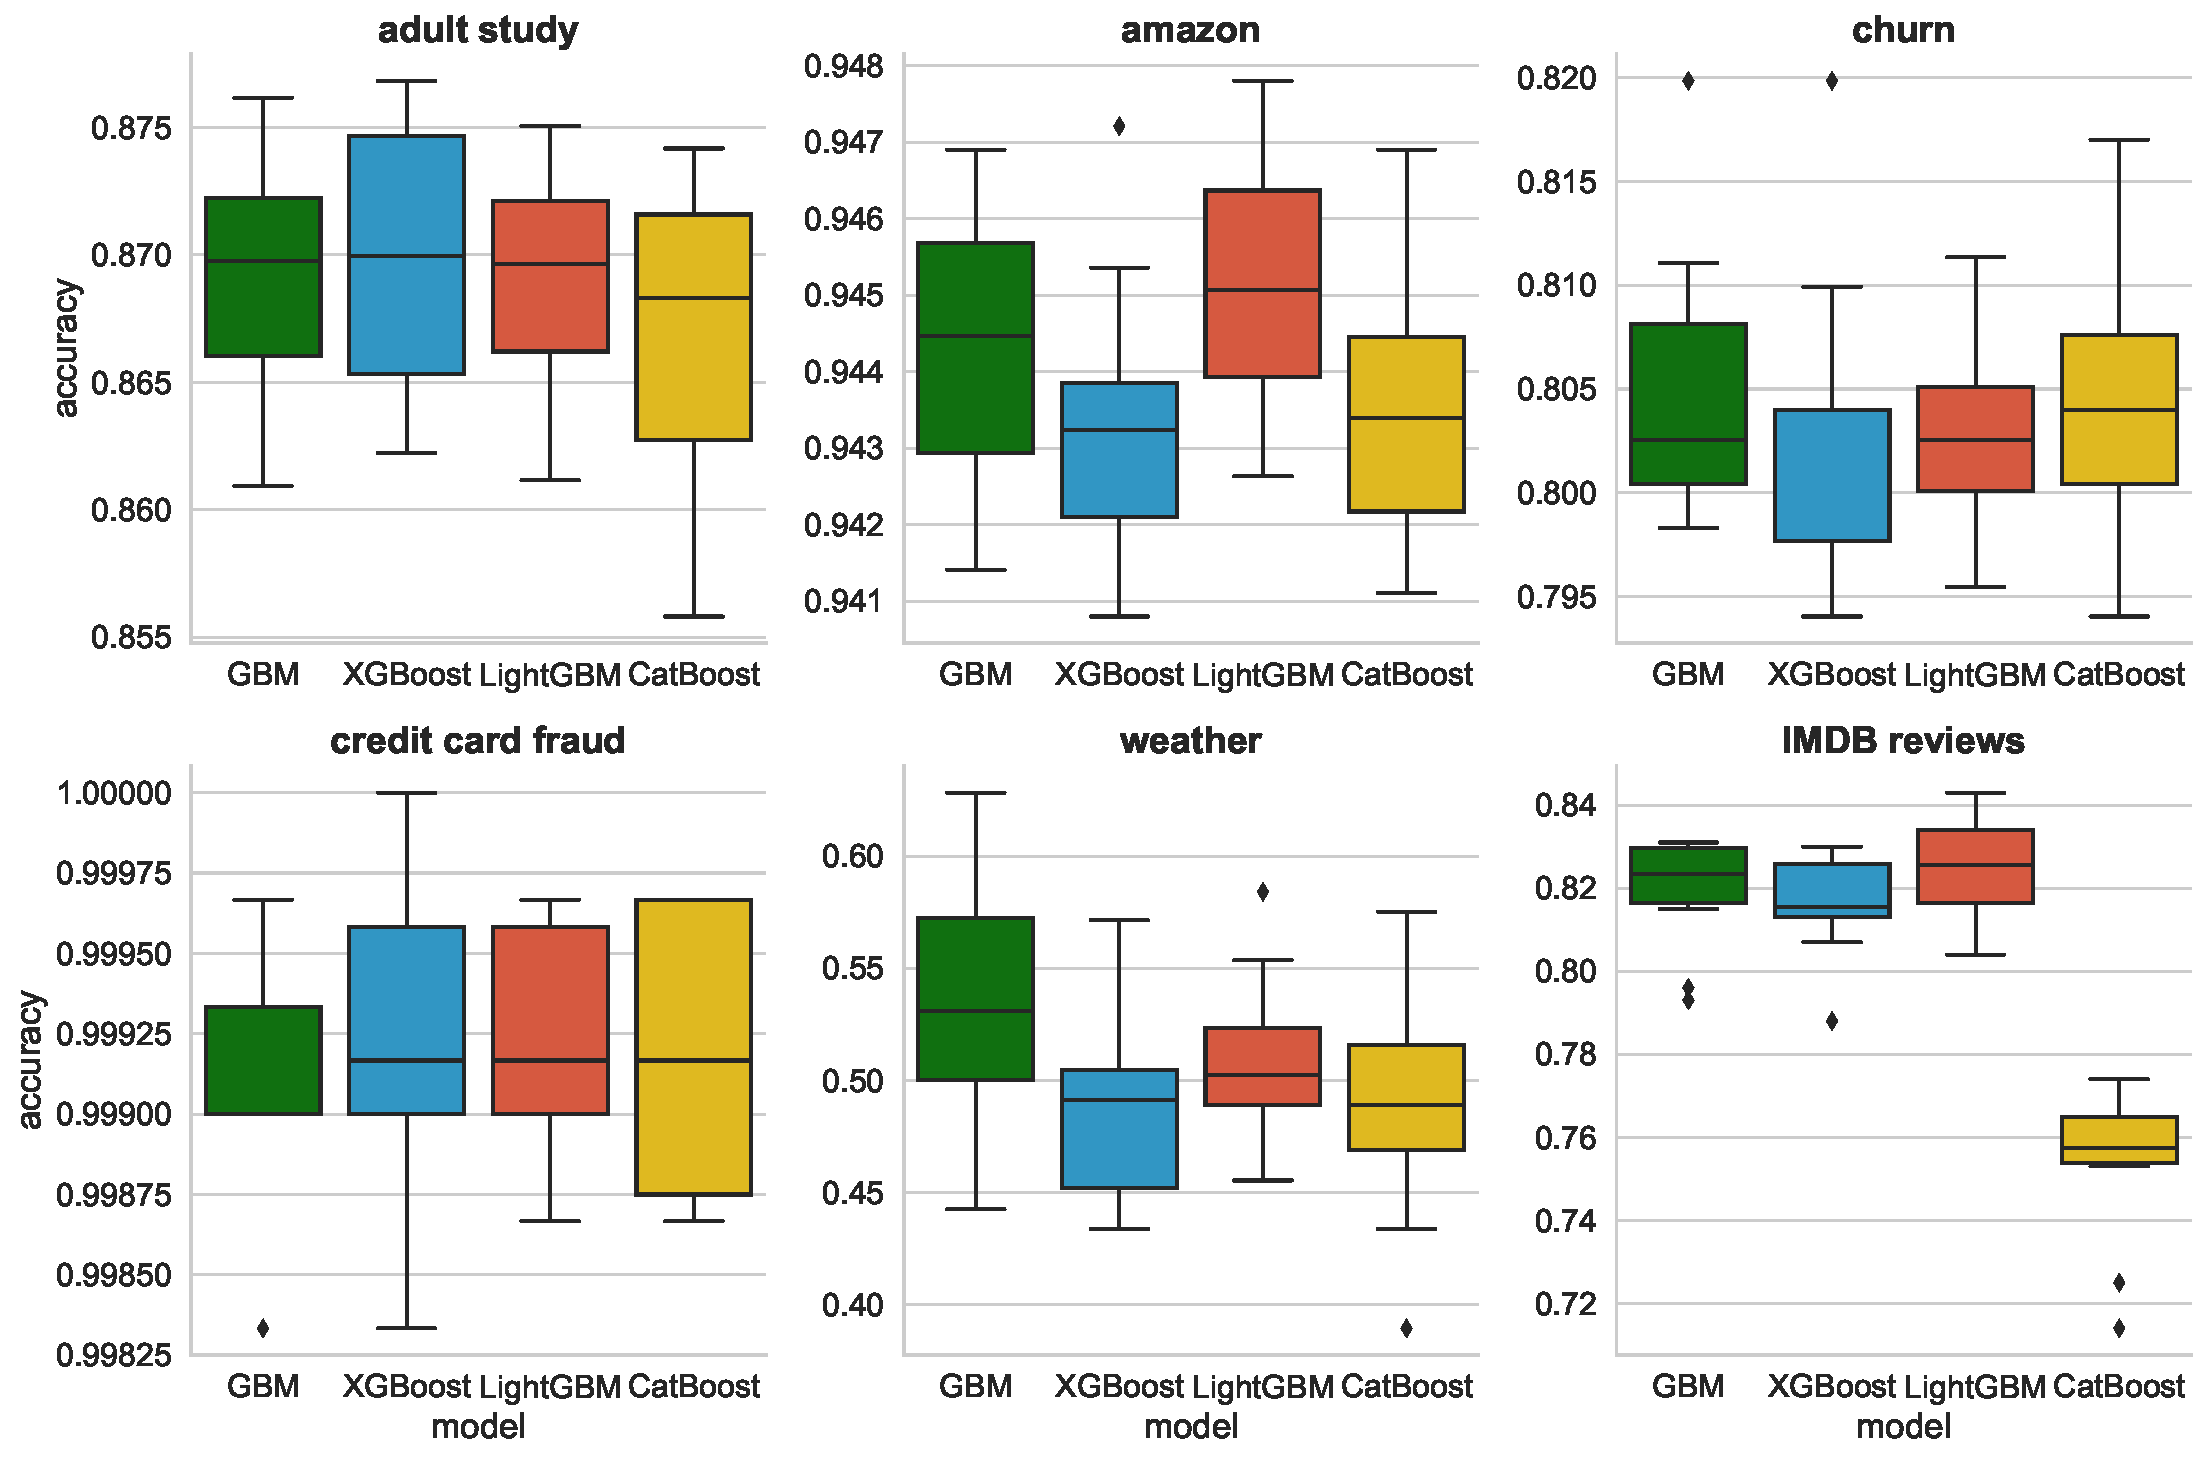
\includegraphics{main/plots/results_accuracy_12_datasets_TPE_150_50_trees_facet.pdf}}
	\caption{Accuracy distributions across 12 datasets with TPE tuning}
	\label{fig:tpe_accuracy}
\end{figure}

Immediately, a vast improvement of gradient boosting and LightGBM can be noticed. Both of the models benefited greatly from hyperparameter tuning and right now all four models: \gbm perform very similarly. Moreover, big increase in LightGBM can be observed; corresponding red boxes are much shorter --- it is possible that the addition of regularization has contributed to lesser spread of accuracy values. A visual judgment would suggest that among tuned models, LightGBM performs the best. XGBoost is also quite robust, but CatBoost seems to have degraded in performance --- even the original GBM proposed by Friedman in 1999 \cite{friedman_gbm} seem to holistically outperform it. The means and standard deviations of accuracy distributions for each model and dataset have been presented in Table~\ref{tab:tpe_accuracy}.

\begin{table}[h!]
\centering
\begin{tabular}{|c|c|c|c|c|}
\hline
\textbf{dataset}  & \textbf{GBM}  & \textbf{XGBoost}  & \textbf{LightGBM}  & \textbf{CatBoost} \\ \hline
adult study & 0.869 $\pm$ 0.005 & \cellcolor{green}0.87 $\pm$ 0.006 & 0.869 $\pm$ 0.005 & \cellcolor{red}0.867 $\pm$ 0.006\\ \hline
heart disease & \cellcolor{red}0.815 $\pm$ 0.086 & 0.828 $\pm$ 0.082 & 0.835 $\pm$ 0.061 & \cellcolor{green}0.838 $\pm$ 0.056\\ \hline
amazon & 0.944 $\pm$ 0.002 & \cellcolor{red}0.943 $\pm$ 0.002 & \cellcolor{green}0.945 $\pm$ 0.002 & \cellcolor{red}0.943 $\pm$ 0.002\\ \hline
mushrooms & 1.0 $\pm$ 0.0 & 1.0 $\pm$ 0.0 & 1.0 $\pm$ 0.0 & 1.0 $\pm$ 0.0\\ \hline
breast cancer & \cellcolor{red}0.963 $\pm$ 0.024 & 0.965 $\pm$ 0.023 & 0.97 $\pm$ 0.02 & \cellcolor{green}0.972 $\pm$ 0.03\\ \hline
churn & \cellcolor{green}0.805 $\pm$ 0.007 & \cellcolor{red}0.803 $\pm$ 0.007 & 0.803 $\pm$ 0.004 & 0.804 $\pm$ 0.007\\ \hline
credit card fraud & 0.999 $\pm$ 0.0 & 0.999 $\pm$ 0.0 & 0.999 $\pm$ 0.0 & 0.999 $\pm$ 0.0\\ \hline
prostate & \cellcolor{green}0.95 $\pm$ 0.071 & 0.94 $\pm$ 0.07 & \cellcolor{red}0.94 $\pm$ 0.084 & \cellcolor{green}0.95 $\pm$ 0.071\\ \hline
leukemia & \cellcolor{red}0.918 $\pm$ 0.098 & 0.932 $\pm$ 0.098 & 0.932 $\pm$ 0.098 & \cellcolor{green}0.973 $\pm$ 0.057\\ \hline
gina agnostic & 0.939 $\pm$ 0.012 & 0.937 $\pm$ 0.014 & \cellcolor{green}0.941 $\pm$ 0.014 & \cellcolor{red}0.911 $\pm$ 0.02\\ \hline
weather & \cellcolor{green}0.537 $\pm$ 0.058 & \cellcolor{red}0.486 $\pm$ 0.042 & 0.51 $\pm$ 0.037 & 0.491 $\pm$ 0.055\\ \hline
IMDB reviews & 0.819 $\pm$ 0.014 & 0.816 $\pm$ 0.013 & \cellcolor{green}0.825 $\pm$ 0.013 & \cellcolor{red}0.753 $\pm$ 0.019\\ \hline
\end{tabular}
\caption{Means and standard deviations of accuracy distributions presented in Figure~\ref{fig:tpe_accuracy}}
\label{tab:tpe_accuracy}
\end{table}

The results in case of AUC have been presented in Figure~\ref{fig:tpe_AUC}.

\begin{figure}[H]
	\centering
		\scalebox{0.42}{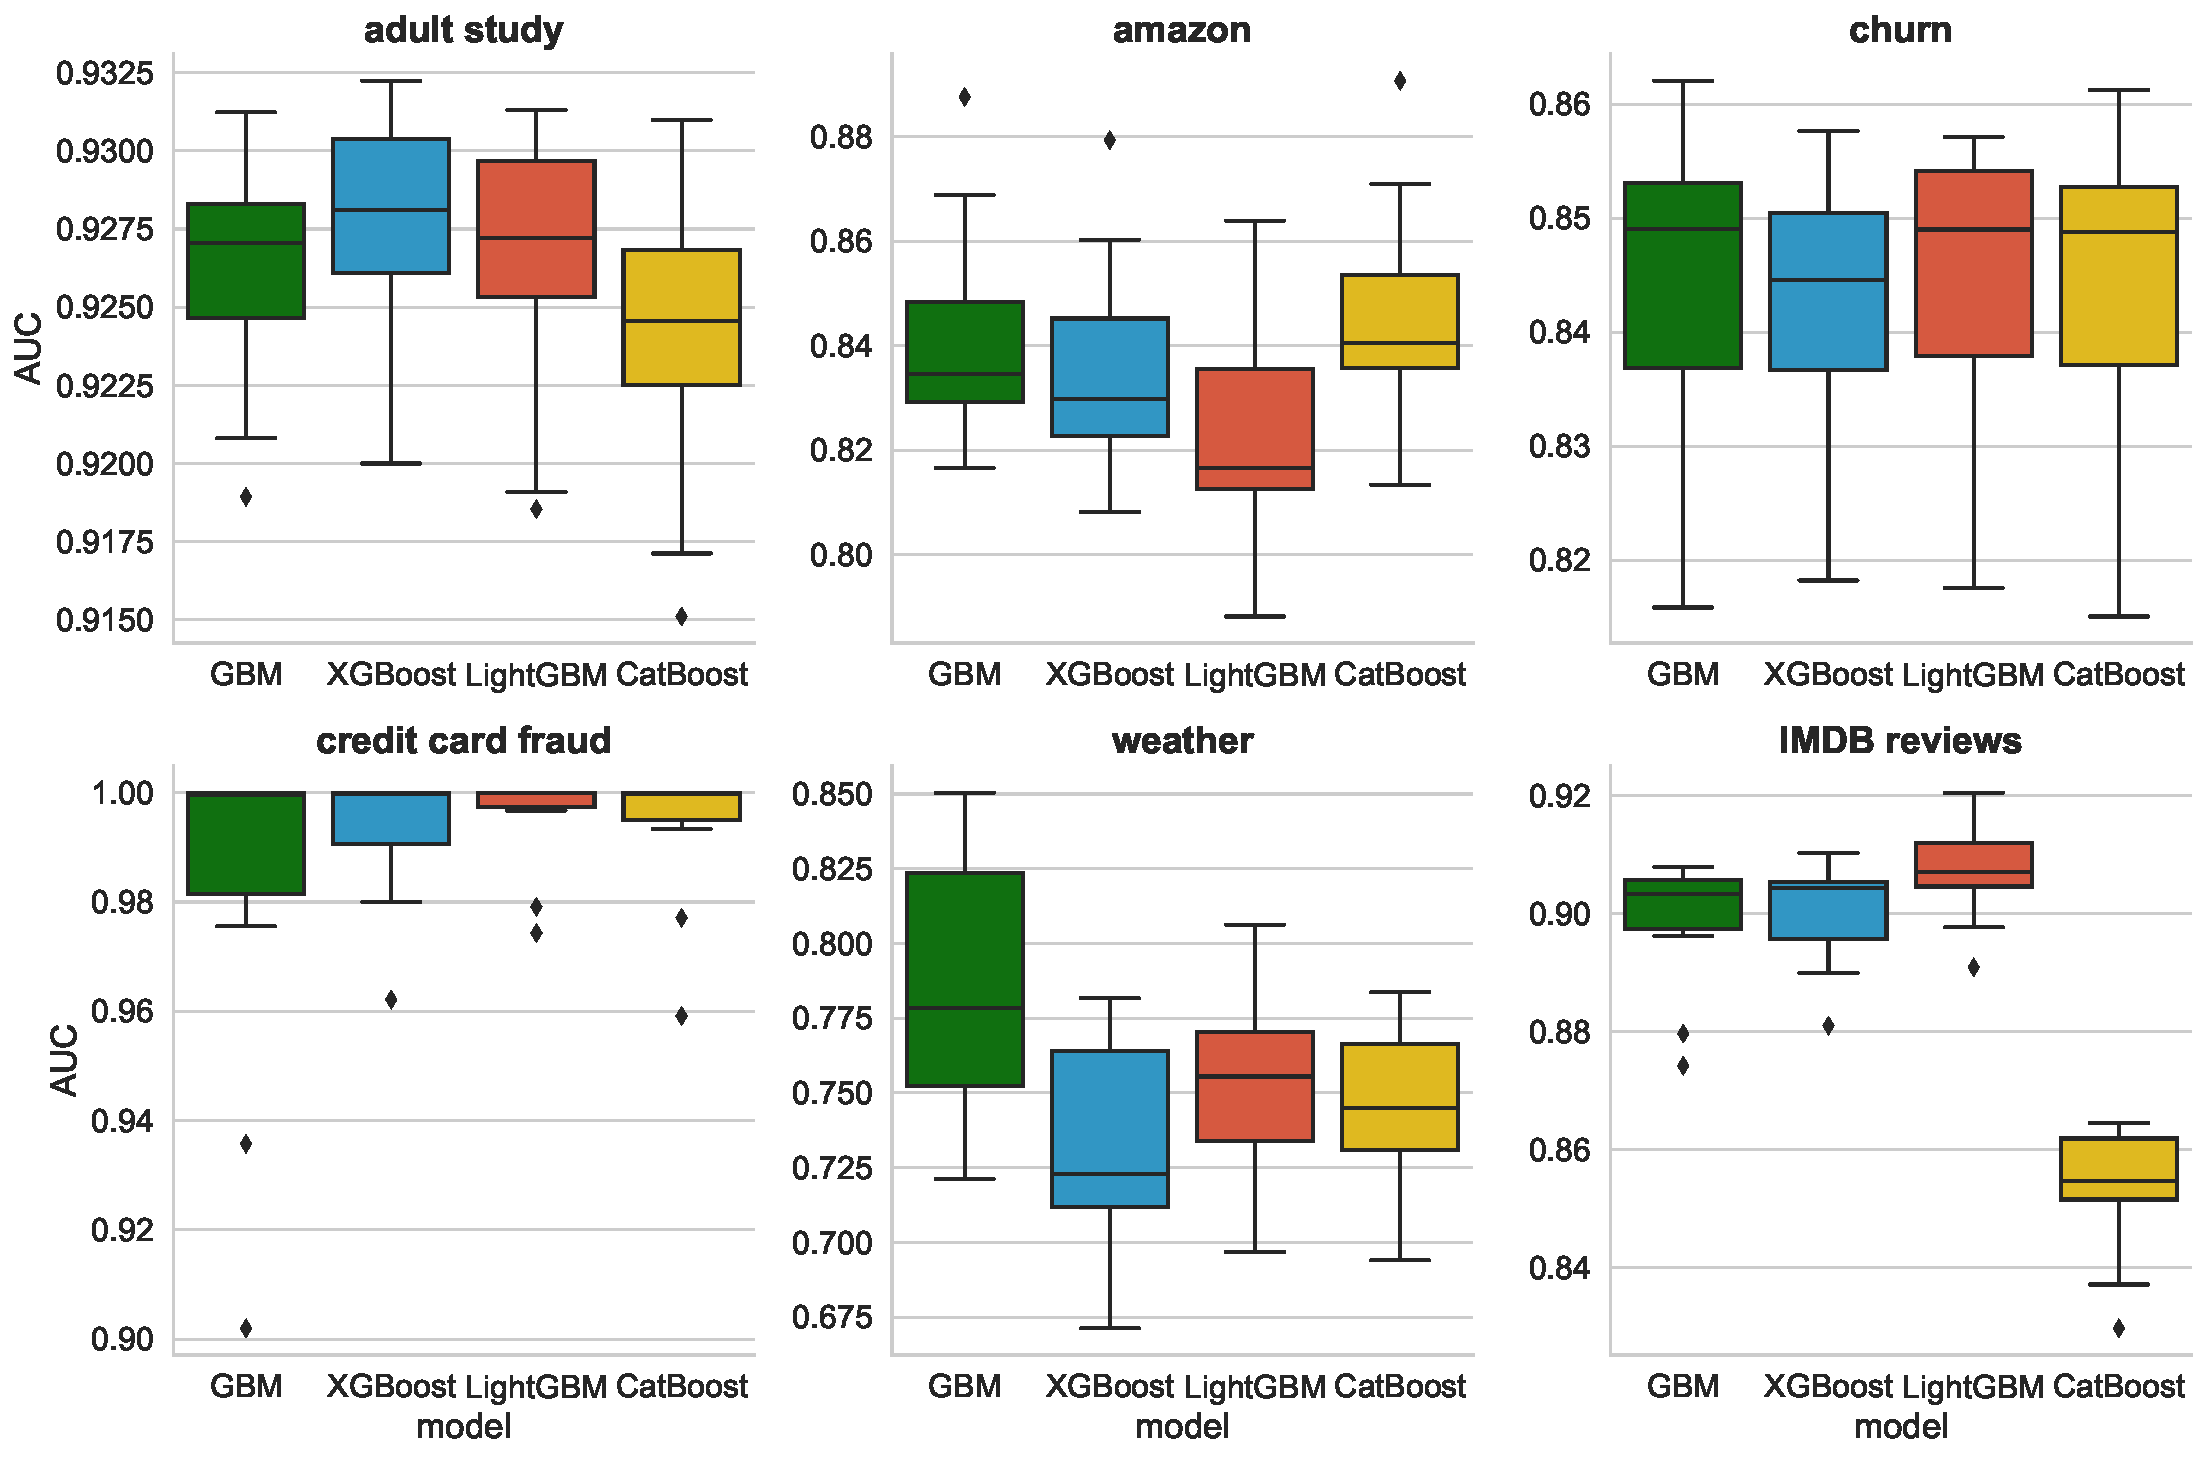
\includegraphics{main/plots/results_AUC_12_datasets_TPE_150_50_trees_facet.pdf}}
	\caption{AUC distributions across 12 datasets with TPE tuning}
	\label{fig:tpe_AUC}
\end{figure}

In terms of accuracy, LightGBM seems to be the most consistent, in case of some datasets it performs the best and it is the worst only on the \emph{prostate} dataset (since LightGBM is tied with XGBoost when considering the means, its accuracy has higher standard deviation). Numerical results confirm that GBM and CatBoost perform very similarly. 
Results for means and standard deviations of AUC have been presented in Table~\ref{tab:tpe_AUC}.

\begin{table}[h!]
\centering
\begin{tabular}{|c|c|c|c|c|}
\hline
\textbf{dataset}  & \textbf{GBM}  & \textbf{XGBoost}  & \textbf{LightGBM}  & \textbf{CatBoost} \\ \hline
adult study & 0.926 $\pm$ 0.004 & \cellcolor{green}0.927 $\pm$ 0.004 & 0.926 $\pm$ 0.004 & \cellcolor{red}0.924 $\pm$ 0.005\\ \hline
heart disease & \cellcolor{red}0.895 $\pm$ 0.062 & 0.899 $\pm$ 0.056 & \cellcolor{green}0.914 $\pm$ 0.055 & 0.906 $\pm$ 0.051\\ \hline
amazon & 0.842 $\pm$ 0.022 & 0.835 $\pm$ 0.022 & \cellcolor{red}0.822 $\pm$ 0.024 & \cellcolor{green}0.845 $\pm$ 0.023\\ \hline
mushrooms & 1.0 $\pm$ 0.0 & 1.0 $\pm$ 0.0 & 1.0 $\pm$ 0.0 & 1.0 $\pm$ 0.0\\ \hline
breast cancer & \cellcolor{red}0.993 $\pm$ 0.012 & 0.994 $\pm$ 0.01 & \cellcolor{green}0.995 $\pm$ 0.01 & 0.994 $\pm$ 0.011\\ \hline
churn & 0.845 $\pm$ 0.014 & \cellcolor{red}0.843 $\pm$ 0.012 & \cellcolor{green}0.845 $\pm$ 0.013 & 0.844 $\pm$ 0.014\\ \hline
credit card fraud & \cellcolor{red}0.981 $\pm$ 0.035 & 0.993 $\pm$ 0.013 & \cellcolor{green}0.995 $\pm$ 0.01 & 0.993 $\pm$ 0.014\\ \hline
prostate & \cellcolor{green}0.968 $\pm$ 0.062 & 0.968 $\pm$ 0.075 & 0.964 $\pm$ 0.076 & \cellcolor{red}0.952 $\pm$ 0.08\\ \hline
leukemia & \cellcolor{red}0.973 $\pm$ 0.064 & 0.98 $\pm$ 0.063 & 0.977 $\pm$ 0.063 & \cellcolor{green}0.99 $\pm$ 0.032\\ \hline
gina agnostic & 0.985 $\pm$ 0.005 & 0.983 $\pm$ 0.005 & \cellcolor{green}0.986 $\pm$ 0.005 & \cellcolor{red}0.971 $\pm$ 0.009\\ \hline
weather & \cellcolor{green}0.786 $\pm$ 0.043 & \cellcolor{red}0.732 $\pm$ 0.036 & 0.754 $\pm$ 0.033 & 0.745 $\pm$ 0.029\\ \hline
IMDB reviews & 0.898 $\pm$ 0.012 & 0.9 $\pm$ 0.009 & \cellcolor{green}0.908 $\pm$ 0.009 & \cellcolor{red}0.853 $\pm$ 0.012\\ \hline
\end{tabular}
\caption{Means and standard deviations of AUC distributions presented in Figure~\ref{fig:tpe_AUC}}
\label{tab:tpe_AUC}
\end{table}

LightGBM is clearly the best when considering AUC scores. The means for each dataset are often the highest and standard deviations are the lowest. Tuned versions of \gbm tend to perform very similarly on the datasets with low to medium number of features, however, some differenced can be observed on highly dimensional datasets. CatBoost's performance there is quite worrying, on the other hand LightGBM handles sparse data (\emph{gina agnostic} and \emph{IMDB reviews} datasets) the best (most likely due to the sparsity-aware splitting algorithm alongside with Exclusive Feature Bundling).

Overall, it can be concluded that hyperparameter tuning using bayesian optimization has leveled out the performances of each of the gradient boosting implementation. However, it is not certain whether if tuned models are actually better than the baseline ones presented in Section~\ref{section:baseline}. The differences of accuracy and AUC scores between the tuned and non-tuned variants of \gbm have been presented in  Tablex~\ref{tab:no_tuning_tpe_accuracy_diff} and ~\ref{tab:no_tuning_tpe_AUC_diff}, respectively.

   \begin{sidewaystable}
     \centering
     \begin{tabular}{c|cccccccc}
\hline
\textbf{dataset} &
\textbf{\begin{tabular}[c]{@{}c@{}}GBM\\ mean\end{tabular}} &
\textbf{\begin{tabular}[c]{@{}c@{}}GBM\\ sdev\end{tabular}} &
\textbf{\begin{tabular}[c]{@{}c@{}}XGBoost\\ mean\end{tabular}} &
\textbf{\begin{tabular}[c]{@{}c@{}}XGBoost\\ sdev\end{tabular}} &
\textbf{\begin{tabular}[c]{@{}c@{}}LightGBM\\ mean\end{tabular}} &
\textbf{\begin{tabular}[c]{@{}c@{}}LightGBM\\ sdev\end{tabular}} &
\textbf{\begin{tabular}[c]{@{}c@{}}CatBoost\\ mean\end{tabular}} &
\textbf{\begin{tabular}[c]{@{}c@{}}CatBoost\\ sdev\end{tabular}} \\ \hline
adult study & +0.225\% & -10.035\% & +0.36\% & +38.802\% & +0.209\% & +18.611\% & -0.465\% & +18.35\%\\ \hline
heart disease & +2.893\% & -14.776\% & +2.395\% & -7.015\% & +0.805\% & +0.007\% & -0.383\% & -0.975\%\\ \hline
amazon & +0.068\% & +45.611\% & -0.2\% & +10.491\% & +0.084\% & +45.447\% & -0.052\% & +87.512\%\\ \hline
mushrooms & 0.0\% & 0.0\% & 0.0\% & 0.0\% & 0.0\% & 0.0\% & +0.012\% & -100.0\%\\ \hline
breast cancer & 0.0\% & +6.5\% & -0.901\% & -1.527\% & +0.363\% & -15.385\% & +0.181\% & +9.296\%\\ \hline
churn & +0.532\% & +32.333\% & +2.204\% & -24.691\% & +3.213\% & -46.033\% & +0.515\% & -23.365\%\\ \hline
credit card fraud & +0.037\% & -34.581\% & -0.003\% & +1.411\% & +0.291\% & -88.242\% & +0.01\% & +0.927\%\\ \hline
prostate & +3.261\% & -10.358\% & 0.0\% & 0.0\% & +6.818\% & -25.722\% & 0.0\% & 0.0\%\\ \hline
leukemia & +8.439\% & -22.171\% & -1.509\% & +1.802\% & +3.162\% & +3.705\% & 0.0\% & 0.0\%\\ \hline
gina agnostic & +2.39\% & -38.174\% & -1.276\% & +6.957\% & -0.579\% & +45.392\% & -3.277\% & +51.498\%\\ \hline
weather & +6.331\% & +54.748\% & -8.215\% & +4.31\% & +1.234\% & -29.377\% & -0.897\% & +15.341\%\\ \hline
IMDB reviews & +6.169\% & +43.014\% & -0.694\% & +21.516\% & +0.279\% & +11.814\% & -8.401\% & +38.744\%\\ \hline
\end{tabular}
\caption{Percentage gain/loss of values of means and standard deviations of accuracy --- TPE tuning vs no tuning}
\label{tab:no_tuning_tpe_accuracy_diff}

    \vspace{1.5\baselineskip}
     \centering
     \begin{tabular}{c|cccccccc}
\hline
\textbf{dataset} &
\textbf{\begin{tabular}[c]{@{}c@{}}GBM\\ mean\end{tabular}} &
\textbf{\begin{tabular}[c]{@{}c@{}}GBM\\ sdev\end{tabular}} &
\textbf{\begin{tabular}[c]{@{}c@{}}XGBoost\\ mean\end{tabular}} &
\textbf{\begin{tabular}[c]{@{}c@{}}XGBoost\\ sdev\end{tabular}} &
\textbf{\begin{tabular}[c]{@{}c@{}}LightGBM\\ mean\end{tabular}} &
\textbf{\begin{tabular}[c]{@{}c@{}}LightGBM\\ sdev\end{tabular}} &
\textbf{\begin{tabular}[c]{@{}c@{}}CatBoost\\ mean\end{tabular}} &
\textbf{\begin{tabular}[c]{@{}c@{}}CatBoost\\ sdev\end{tabular}} \\ \hline
adult study & +0.281\% & -15.696\% & +0.141\% & +3.778\% & +0.281\% & -2.272\% & -0.518\% & +23.227\%\\ \hline
heart disease & +2.207\% & -3.913\% & +2.39\% & +0.236\% & +1.201\% & +4.594\% & +0.75\% & -7.96\%\\ \hline
amazon & +2.837\% & +13.254\% & +1.226\% & +16.862\% & -0.704\% & +14.502\% & +1.609\% & +7.323\%\\ \hline
mushrooms & 0.0\% & +216.228\% & 0.0\% & -100.0\% & 0.0\% & 0.0\% & 0.0\% & -100.0\%\\ \hline
breast cancer & -0.112\% & +9.288\% & -0.027\% & +2.344\% & +0.159\% & -31.696\% & +0.053\% & -9.179\%\\ \hline
churn & +0.688\% & +18.875\% & +3.18\% & -4.343\% & +3.805\% & -8.839\% & +0.565\% & -3.227\%\\ \hline
credit card fraud & +5.143\% & -51.348\% & +0.466\% & -37.012\% & +23.897\% & -95.758\% & +0.48\% & -31.941\%\\ \hline
prostate & +2.542\% & -25.0\% & +0.415\% & +17.47\% & 0.0\% & +73.734\% & -0.833\% & +2.326\%\\ \hline
leukemia & +2.277\% & -17.382\% & 0.0\% & 0.0\% & +0.861\% & -3.154\% & -1.0\% & 0\%\\ \hline
gina agnostic & +1.333\% & -22.642\% & -0.405\% & +11.921\% & +0.014\% & +15.313\% & -1.296\% & +68.488\%\\ \hline
weather & +4.62\% & +35.32\% & -5.549\% & -23.271\% & +0.138\% & -20.273\% & -0.432\% & -23.948\%\\ \hline
IMDB reviews & +4.211\% & +9.168\% & -0.315\% & -0.261\% & +0.084\% & -7.264\% & -5.938\% & +15.504\%\\ \hline
\end{tabular}
\caption{Percentage gain/loss of values of means and standard deviations of AUC --- TPE tuning vs no tuning}
\label{tab:no_tuning_tpe_AUC_diff}
   \end{sidewaystable}
   
When looking at the change of mean values of accuracy and AUC one can notice that tuning
It can be noticed that TPE tuning has increased the performance of \gbm in terms of the mean values. The absolute value of the means in case of accuracy and AUC usually does not exceed 10\%. The most negative change of mean has been observed in the case of CatBoost's accuracy on the \emph{IMDB reviews} dataset --- TPE tuning has decreased the performance of the model by around 8.4\%. On the other hand, the biggest gain has been recorded in case of LightGBM. Mean AUC on the \emph{credit card fraud} dataset has increased by almost 24\%. On the other hand, standard deviations changed much more drastically, either positively or negatively. After TPE tuning, the standard deviations have to be considered on case-by-case basis, one model and one dataset at a time. Similar conclusions can be drawn by considering F1 score instead of accuracy or AUC.

Bayesian optimization in itself is quite slow due to its sequential nature --- tuning times of the algorithms have been presented in Figure~\ref{fig:tpe_tuning_times}.

\begin{figure}[H]
	\centering
		\scalebox{0.42}{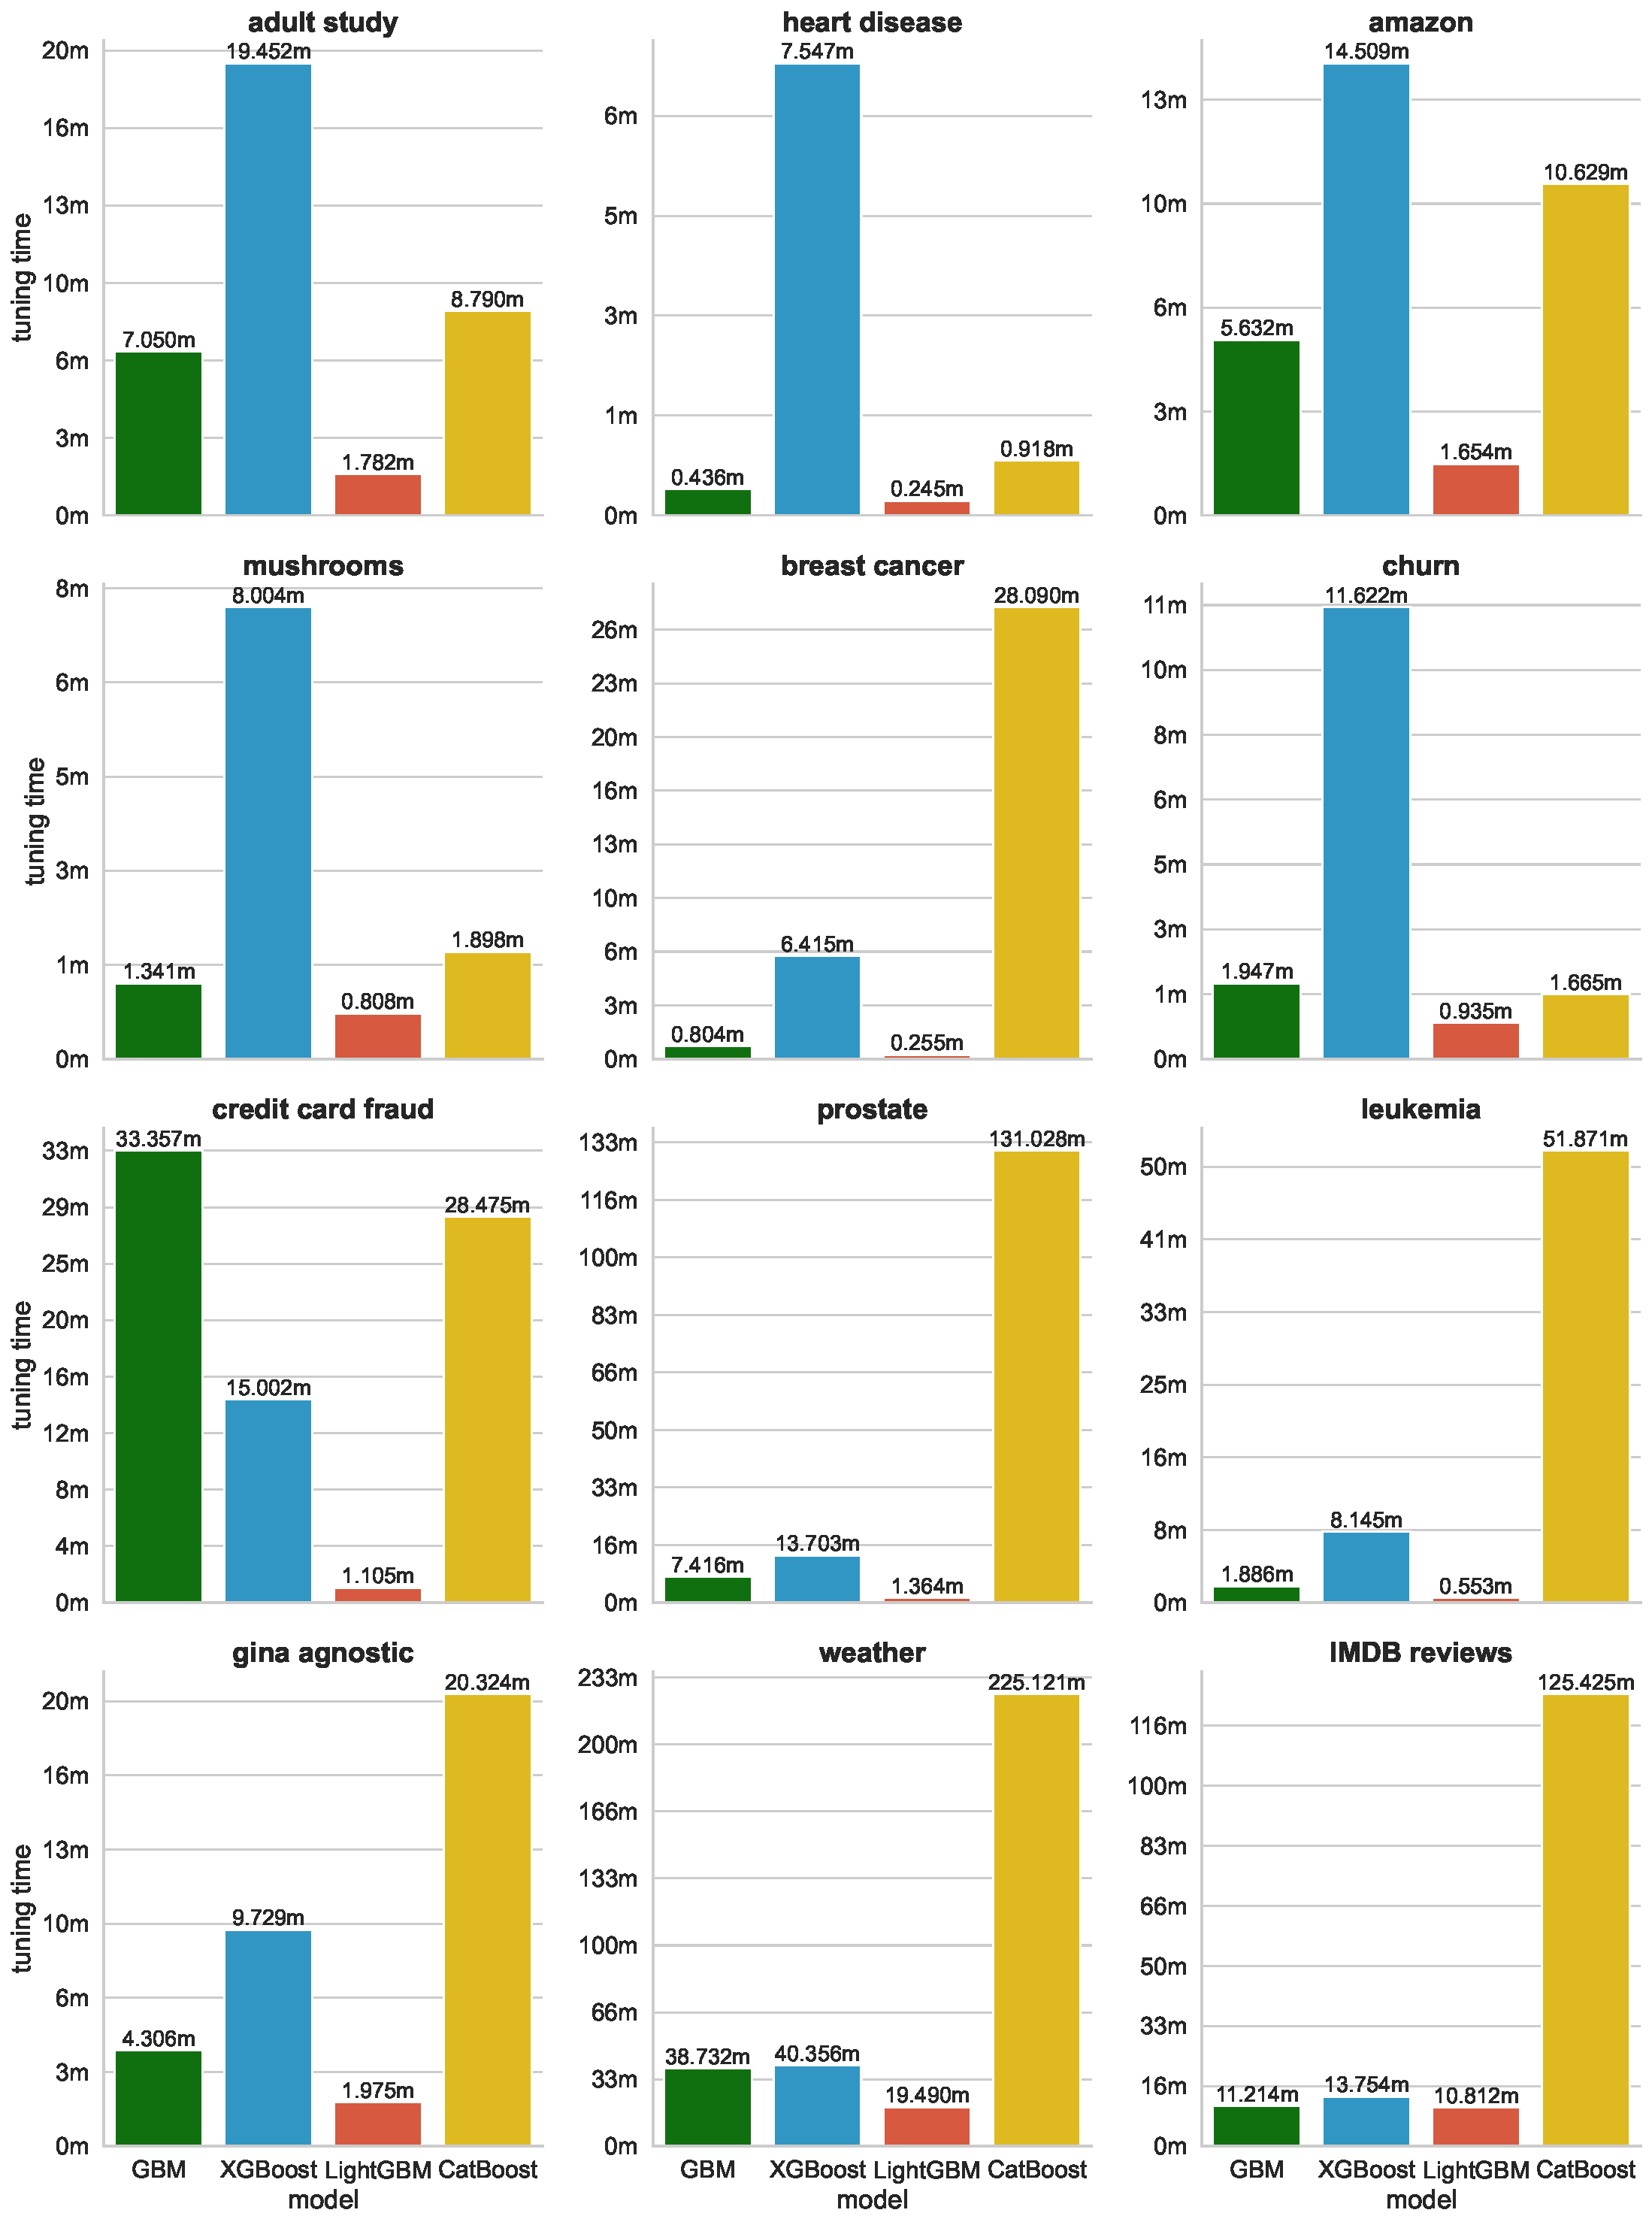
\includegraphics{main/plots/tuning_times_12_datasets_TPE_150_50_trees_facet.pdf}}
	\caption{Tuning times of the models across 12 datasets with TPE tuning}
	\label{fig:tpe_tuning_times}
\end{figure}

Additional time to perform model selection is quite long --- in the case of datasets with a reasonable number of features it can be stated that the time consumed to perform hyperparameter tuning is worth the slight increase of models' performance in terms of accuracy, F1 score and AUC. The situation is different on highly dimensional datasets, especially in case of CatBoost which is very inefficient (also for some reason it does not handle the \emph{breast cancer} dataset which is strange). Two or three our long hyperparameter tuning in case of CatBoost is not worth the time spent, especially that in the case of the \emph{IMDB reviews} dataset the tuning was actually detrimental. On the other hand, GBM seems to be quite fast, XGBoost is slightly less consistent. The algorithm which benefited the most from the tuning is also the most efficient --- LightGBM is lightning fast. The difference of the tuning times compared to other models is enormous --- the tuning times are often lower by one or two orders of magnitude. The difference is the biggest in the case of the \emph{breast cancer} dataset; LightGBM is over 100 times faster (in other words, one could perform TPE tuning over the span of 1500 iterations instead of 15 and there is a high chance that LightGBM would still complete the tuning process faster than CatBoost). It can be stated that LightGBM is the GBM implementation of choice for performing hyperparameter tuning due to a significant increase in performance as well as enormous scalability and efficiency.

The runtimes of the models selected in the hyperparameter tuning have been presented in Figure~\ref{fig:tpe_runtimes}.

\begin{figure}[H]
	\centering
		\scalebox{0.42}{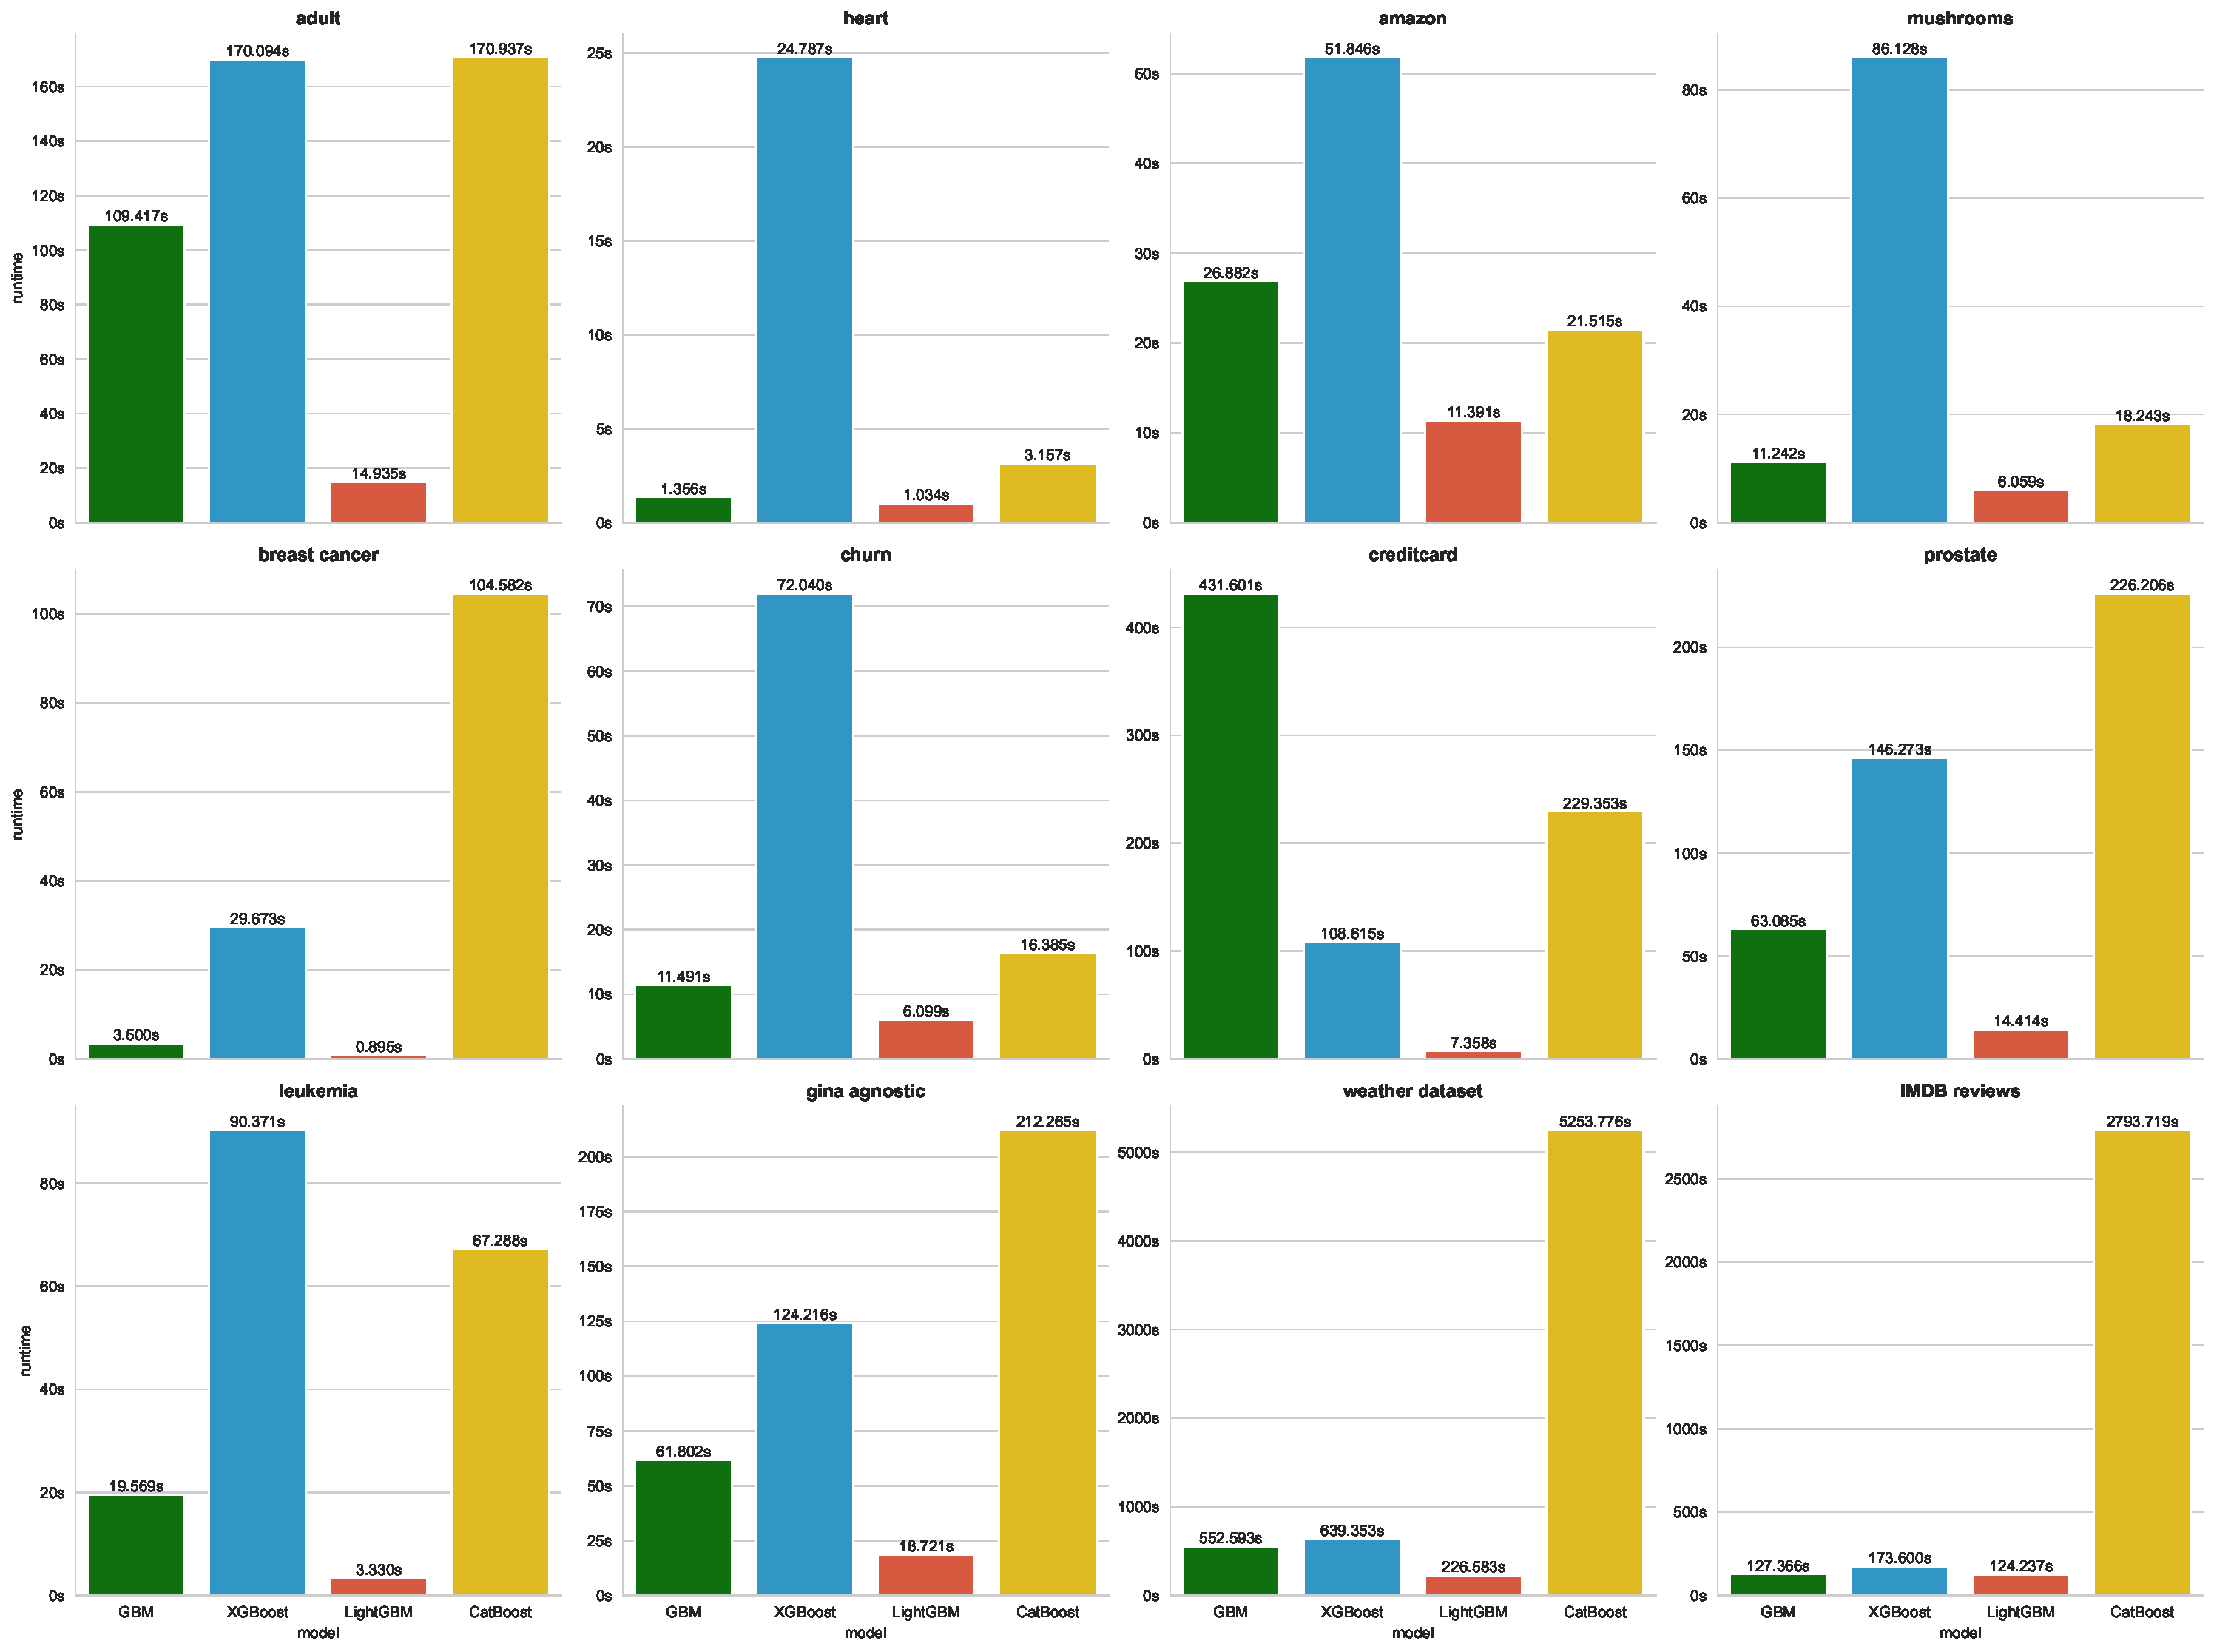
\includegraphics{main/plots/runtimes_12_datasets_TPE_150_50_trees_facet.pdf}}
	\caption{Runtimes of the models across 12 datasets with TPE tuning}
	\label{fig:tpe_runtimes}
\end{figure}

In general, the runtimes of the tuned models are lower than those of baseline ones. Regularization has definitely helped to decrease the runtime, as well as randomization in form of instance and feature subsampling. On the other hand, higher runtimes may be due to the fact that the \emph{max\_depth} hyperparameter was tuned. In some cases, the best model chosen by TPE tuning could grow trees up to 10 levels deep, which would greatly increase the runtime (by default, GBM models use shallower trees with 4-6 levels).

In order to rank \gbm tuned using Tree Parzen Estimators, Friedman test with Nemenyi Post Hoc Analysis has been performed. Ranking in case of F1 score has been presented in Figure~\ref{fig:tpe_F1_heatmap}.

\begin{figure}[H]
	\centering
		\scalebox{0.7}{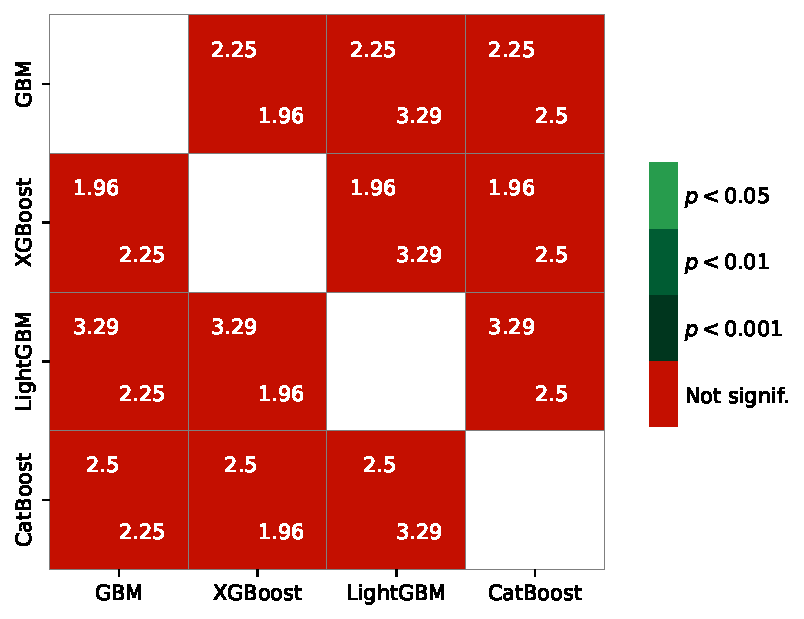
\includegraphics{main/plots/heatmap_f1_score_12_datasets_TPE_150_50_trees.pdf}}
	\caption{Ranking of tuned models' F1 scores. Critical difference $CD = 1.354$}
	\label{fig:tpe_F1_heatmap}
\end{figure}

Every difference in the rankings is lower than the critical difference threshold equal to 1.354. The ranks for GBM, XGBoost and CatBoost are quite close, but LightGBM is ranked much higher. The difference between the worst and the best model --- XGBoost and LightGBM equal to 1.33 which is very close to the critical difference is not statistically significant, but it is apparent that tuned LightGBM is in fact better than tuned XGBoost (the difference in performance can be observed in Figures~\ref{fig:tpe_accuracy}, \ref{fig:tpe_AUC} and Tables~\ref{tab:tpe_accuracy} and \ref{tab:tpe_AUC}). In case of accuracy and AUC metrics, the rankings are similar to the one presented in Figure~\ref{fig:tpe_F1_heatmap}, although all pairwise comparison of models are still statistically significant. 

Finally, it was essential to use the Friedman test with Nemenyi Post Hoc Analysis to determine the rankings of 8 models: the baseline versions of \gbm and their tuned counterparts. From the visual analysis it can be assumed that tuned LightGBM is the best model, overall and baseline gradient boosting is the worst one. The ranking of algorithms excluding the two aforementioned models is not clear --- that is why the Friedman test will help to prepare such ranking in the most objective way. The heatmap with the rankings of performance in terms of AUC of all eight models have been presented in Figure~\ref{fig:no_tuning_tpe_AUC_heatmap}.

\begin{figure}[H]
	\centering
		\scalebox{0.8}{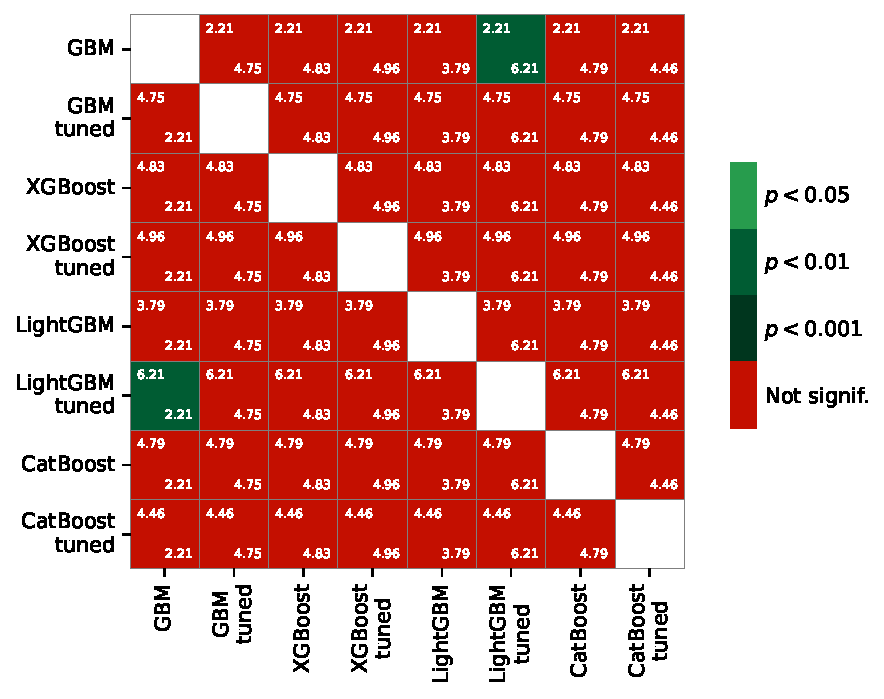
\includegraphics{main/plots/heatmap_AUC_combined_TPE_150_50_trees.pdf}}
	\caption{Ranking of tuned models' F1 scores. Critical difference $CD = 3.031$}
	\label{fig:no_tuning_tpe_AUC_heatmap}
\end{figure}

Friedman test with Nemenyi Post Hoc Analysis implies that there is only one case where the pairwise comparison of rankings of two models is statistically significant --- the performance of tuned LightGBM is statistically different (in this case better) than the performance of baseline GBM. A similar pattern can be observed in the case of rankings obtained for accuracy and F1 score, but in those cases the p-value of the Nemenyi test was higher ($p<0.05$, was $p<0.01$ in case of AUC). In case of all three aforementioned evaluation metrics, the rankings all quite similar --- tuned LightGBM is the best by a big margin in the rank, then models such as XGBoost, tuned XGBoost, CatBoost and tuned CatBoost and tuned GBM can be considered as the next best models (although not always in that particular order), however, the difference in their ranks is quite small. Lastly, two worst algorithms are LightGBM and GBM which is not surprising.   

\subsection{Comparison between randomized search, bayesian optimization and no tuning}\label{section_rand}
In Sections~\ref{section:baseline} and \ref{section_tpe} comparative analysis of baseline and tuned variants of \gbm has been conducted. The method of choice for hyperparameter tuning was bayesian optimization using Tree Parzen Estimators. In this section, a different method used for model selection will be analyzed, namely the randomized search. Bayesian optimization has proven to be effective, but quite time consuming and computationally demanding, thus it is reasonable to check if simpler methods, such as aforementioned randomized search can be a better alternative. 

Each iteration of randomized search is independent from each other one, so the tuning procedure can parallelized --- thus, it is expected that 15 iterations of randomized search will take less time than tuning using Tree Parzen Estimators. Therefore, the number of iterations has been set to 30 --- the differences of tuning times between two aforementioned model selection methods have been presented in Figure~\ref{fig:diffs}.

\begin{figure}[H]
	\centering
		\scalebox{0.42}{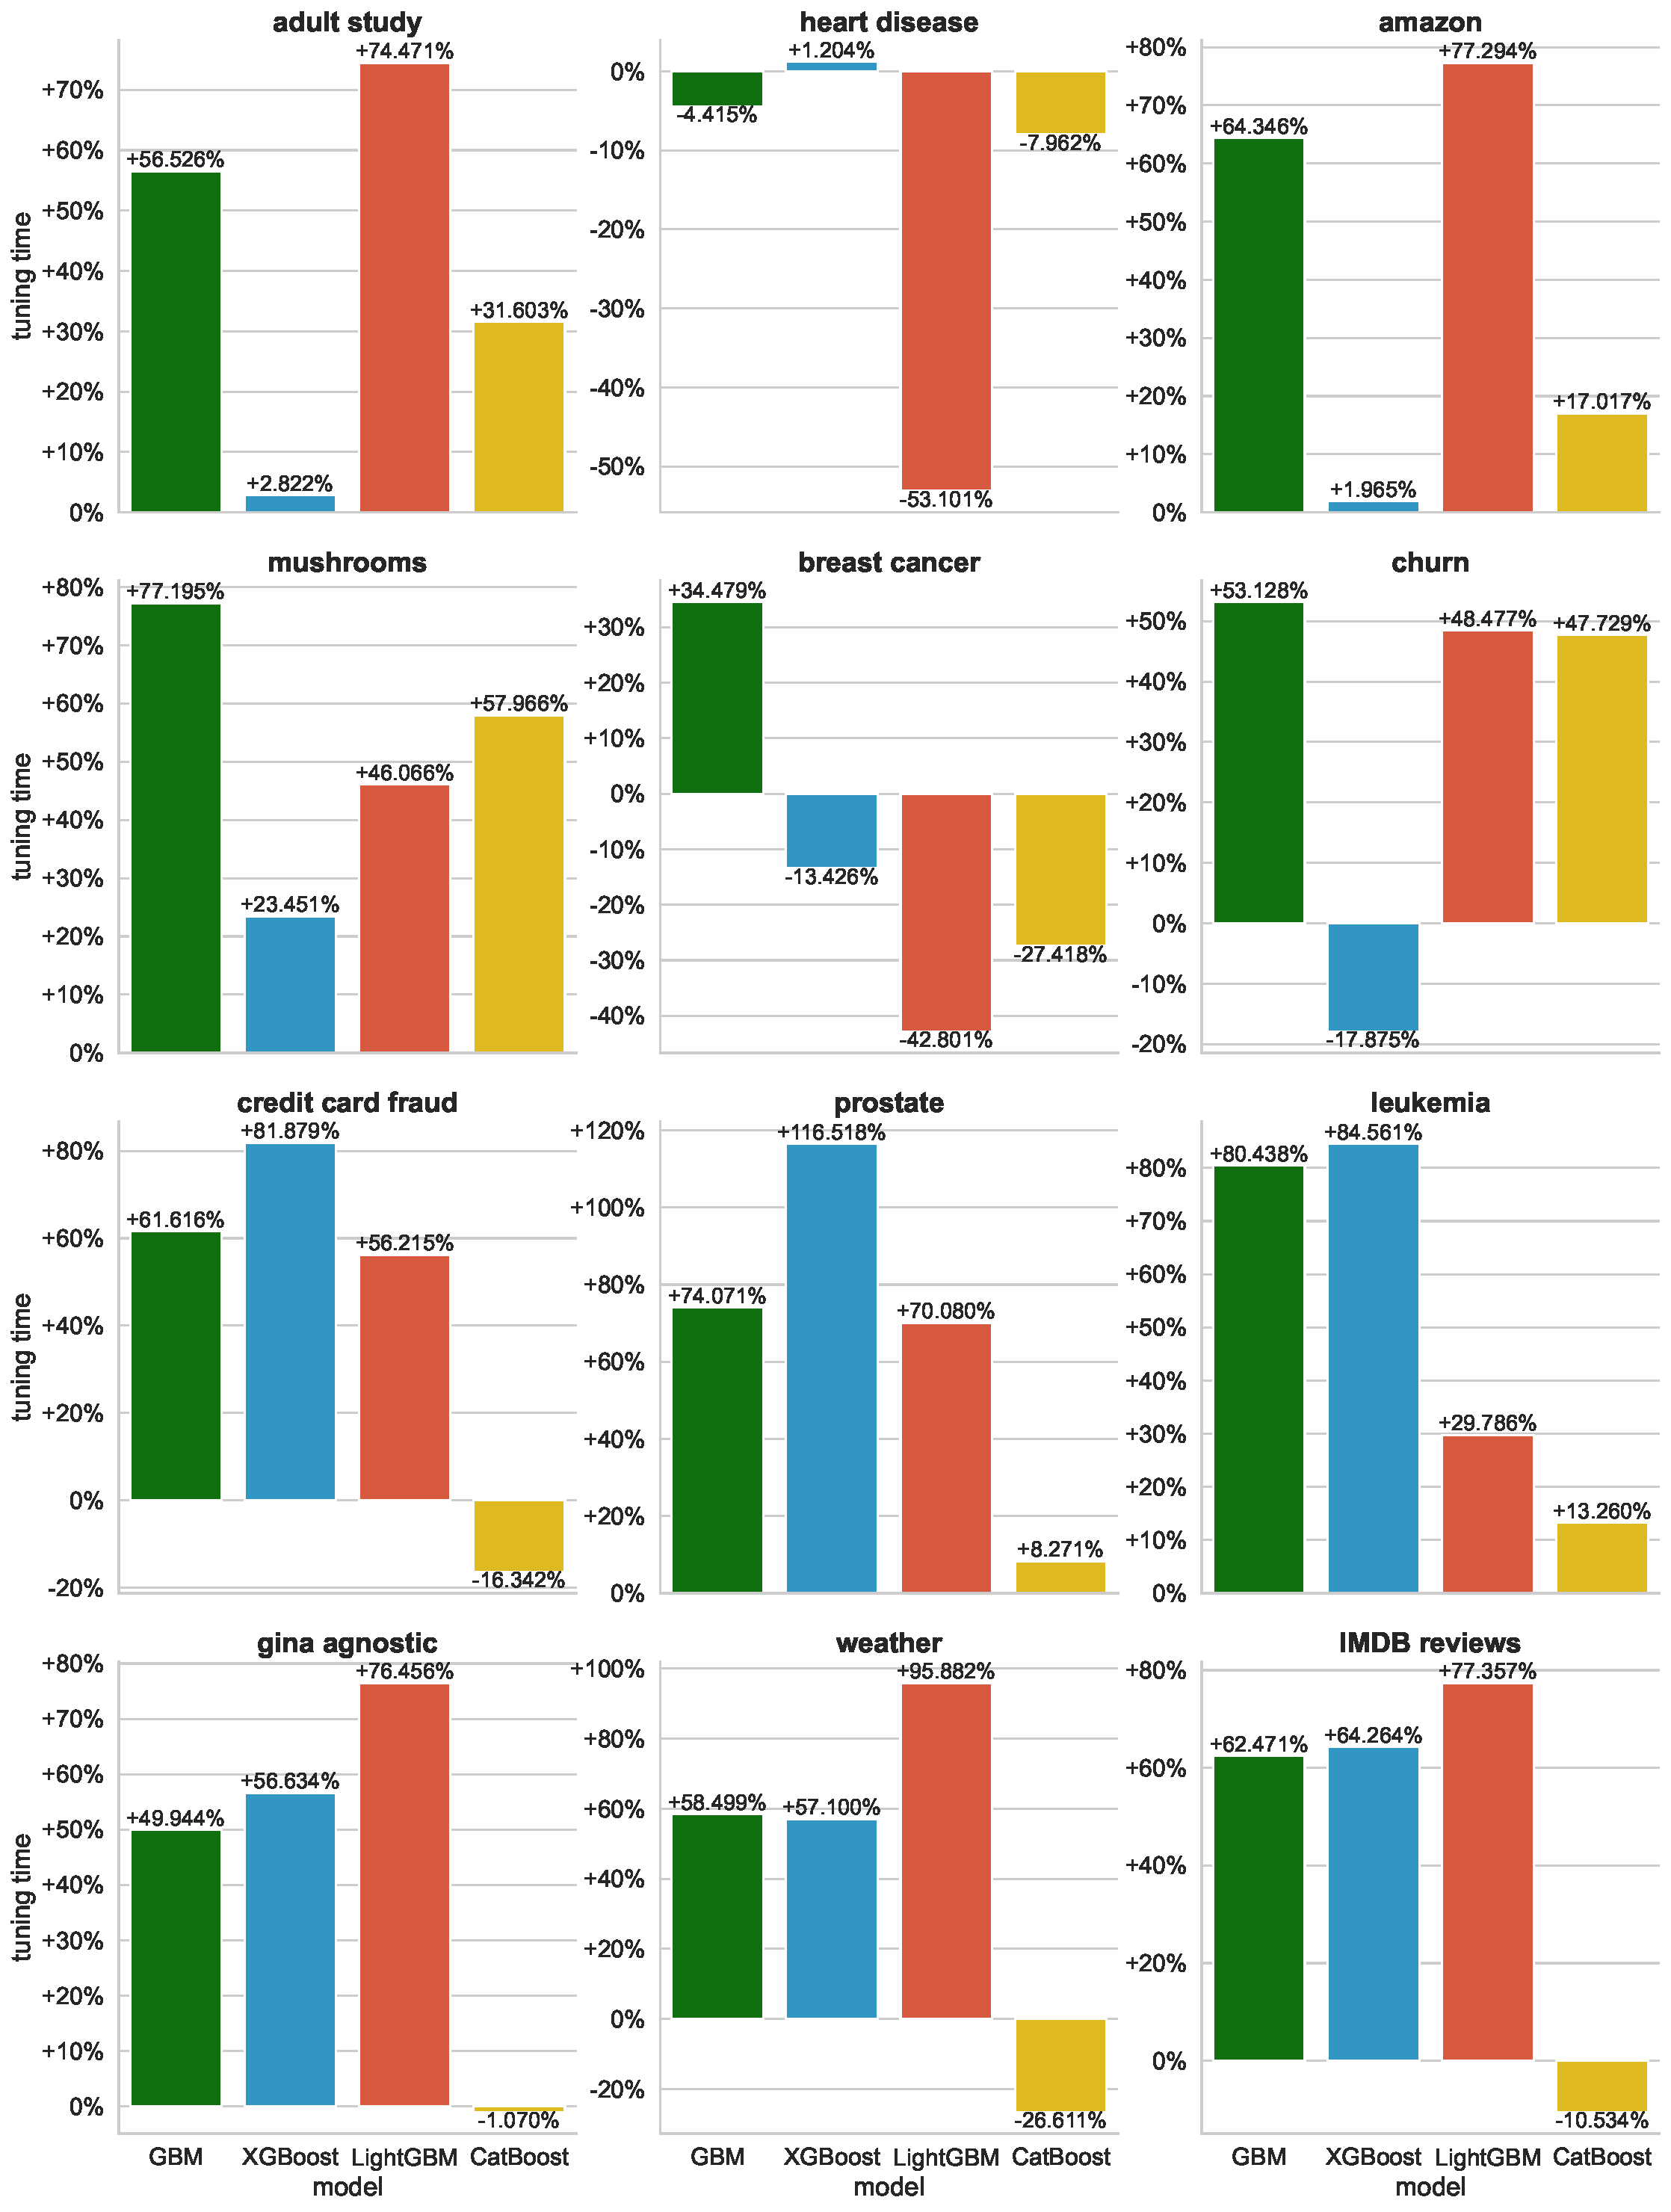
\includegraphics{main/plots/diffs_barplots.pdf}}
	\caption{Differences between tuning times using randomized search and bayesian optimization}
	\label{fig:diffs}
\end{figure}

On most of the datasets, randomized search took longer time than TPE tuning. In some cases the time to complete model selection was longer by over 50\%, but sometimes randomized search was faster. 

It is essential to compare the performance of both types of hyperparameter tuning and the case where there was no tuning performed. The comparison has been performed for each GBM implementation: \gbm and each evaluation metric: accuracy, F1 score and AUC in the following scenarios:

\begin{enumerate}
    \item no tuning vs bayesian optimization using TPE
    \item no tuning vs randomized search
    \item bayesian optimization vs randomized search
\end{enumerate}

All pairwise tests have been performed using the Wilcoxon Signed Rank Test with one-sided alternative hypothesis. The results have been compiled in Table~\ref{tab:no_tuning_tpe_rand}.

\begin{table}[h!]
\centering
\begin{tabular}{|c|c|c|c|c|}
\hline
\textbf{model} & \diagbox{\textbf{metric}}{\textbf{case}}         & \textbf{no tuning | TPE} & \textbf{no tuning | rand.} & \textbf{TPE | rand.} \\ \hline
               & accuracy & TPE                       & randomized                 & $p > 0.05$                 \\ \cline{2-5} 
GBM            & F1 score & TPE                       & randomized                 & $p > 0.05$                 \\ \cline{2-5} 
               & AUC      & TPE                       & randomized                 & $p > 0.05$                 \\ \hline
               & accuracy & $p > 0.05$                      & $p > 0.05$                       & $p > 0.05$                 \\ \cline{2-5} 
XGBoost        & F1 score & $p > 0.05$                      & $p > 0.05$                       & randomized           \\ \cline{2-5} 
               & AUC      & $p > 0.05$                      & $p > 0.05$                       & $p > 0.05$                 \\ \hline
               & accuracy & TPE                       & randomized                 & randomized           \\ \cline{2-5} 
LightGBM       & F1 score & TPE                       & randomized                 & randomized           \\ \cline{2-5} 
               & AUC      & TPE                       & randomized                 & randomized           \\ \hline
               & accuracy & $p > 0.05$                      & $p > 0.05$                       & $p > 0.05$                 \\ \cline{2-5} 
CatBoost       & F1 score & $p > 0.05$                      & $p > 0.05$                       & $p > 0.05$                 \\ \cline{2-5} 
               & AUC      & $p > 0.05$                      & $p > 0.05$                       & $p > 0.05$                 \\ \hline
\end{tabular}
\caption{Comparison of TPE and randomized search tuning in contrast to no tuning}
\label{tab:no_tuning_tpe_rand}
\end{table}

In case of GBM and LightGBM it is always more optimal to perform either TPE tuning or randomized search rather than not. On the other hand, in case of XGBoost and CatBoost no significant differences of performing hyperparameter tuning have been found --- it may imply that XGBoost and CatBoost do not have to be tuned at all.

The comparison between bayesian optimization (15 iterations) and randomized search (30 iterations) is interesting --- the latter has proven to be better than the former when evaluating XGBoost using the F1 score. LightGBM tends to benefit from the randomized search; the usual longer tuning time compared to bayesian optimization is worth it. It may be beneficial to pair TPE tuning with GBM, XGBoost or CatBoost.

Moreover, randomized search with 15 iterations has been tested. Overall, it is much faster than bayesian optimization, but has not proven to be better while using LightGBM.

The final rankings of the models in terms of choice of hyperparameter tuning method and evaluation metric has been presented in Figure~\ref{tab:all_tunings_rankings}. 

%wnioski do tego/obserwacje 
%inne eksperymenty

\newpage
\begin{table}[h!]
\centering
\begin{tabular}{|c|c|c|c|}
\hline
\textbf{\begin{tabular}[c]{@{}c@{}}model\\ rank\end{tabular}} &
  \textbf{accuracy} &
  \textbf{F1 score} &
  \textbf{AUC} \\ \hline
\textbf{\#1} &
  \begin{tabular}[c]{@{}c@{}}LightGBM\\ randomized\\ 9.75\end{tabular} &
  \begin{tabular}[c]{@{}c@{}}LightGBM\\ randomized\\ 9.62\end{tabular} &
  \begin{tabular}[c]{@{}c@{}}LightGBM\\ randomized\\ 9.46\end{tabular} \\ \hline
\textbf{\#2} &
  \begin{tabular}[c]{@{}c@{}}LightGBM\\ TPE\\ 7.54\end{tabular} &
  \begin{tabular}[c]{@{}c@{}}LightGBM\\ TPE\\ 8.25\end{tabular} &
  \begin{tabular}[c]{@{}c@{}}LightGBM\\ TPE\\ 8.38\end{tabular} \\ \hline
\textbf{\#3} &
  \begin{tabular}[c]{@{}c@{}}XGBoost\\ no tuning\\ 7.50\end{tabular} &
  \begin{tabular}[c]{@{}c@{}}CatBoost\\ no tuning\\ 7.54\end{tabular} &
  \begin{tabular}[c]{@{}c@{}}XGBoost\\ randomized\\ 7.21\end{tabular} \\ \hline
\textbf{\#4} &
  \begin{tabular}[c]{@{}c@{}}CatBoost\\ no tuning\\ 7.12\end{tabular} &
  \begin{tabular}[c]{@{}c@{}}XGBoost\\ no tuning\\ 7.50\end{tabular} &
  \begin{tabular}[c]{@{}c@{}}XGBoost\\ TPE\\ 6.88\end{tabular} \\ \hline
\textbf{\#5} &
  \begin{tabular}[c]{@{}c@{}}XGBoost\\ randomized\\ 6.88\end{tabular} &
  \begin{tabular}[c]{@{}c@{}}XGBoost\\ randomized\\ 7.04\end{tabular} &
  \begin{tabular}[c]{@{}c@{}}CatBoost\\ no tuning\\ 6.75\end{tabular} \\ \hline
\textbf{\#6} &
  \begin{tabular}[c]{@{}c@{}}GBM\\ randomized\\ 6.58\end{tabular} &
  \begin{tabular}[c]{@{}c@{}}GBM\\ randomized\\ 6.62\end{tabular} &
  \begin{tabular}[c]{@{}c@{}}XGBoost\\ no tuning\\ 6.54\end{tabular} \\ \hline
\textbf{\#7} &
  \begin{tabular}[c]{@{}c@{}}GBM\\ TPE\\ 6.50\end{tabular} &
  \begin{tabular}[c]{@{}c@{}}GBM\\ TPE\\ 6.17\end{tabular} &
  \begin{tabular}[c]{@{}c@{}}GBM\\ TPE\\ 6.50\end{tabular} \\ \hline
\textbf{\#8} &
  \begin{tabular}[c]{@{}c@{}}CatBoost\\ TPE\\ 6.17\end{tabular} &
  \begin{tabular}[c]{@{}c@{}}CatBoost\\ TPE\\ 6.08\end{tabular} &
  \begin{tabular}[c]{@{}c@{}}CatBoost\\ TPE\\ 6.21\end{tabular} \\ \hline
\textbf{\#9} &
  \begin{tabular}[c]{@{}c@{}}CatBoost\\ randomized\\ 5.71\end{tabular} &
  \begin{tabular}[c]{@{}c@{}}CatBoost\\ randomized\\ 5.50\end{tabular} &
  \begin{tabular}[c]{@{}c@{}}GBM\\ randomized\\ 6.12\end{tabular} \\ \hline
\textbf{\#10} &
  \begin{tabular}[c]{@{}c@{}}XGBoost\\ TPE\\ 5.54\end{tabular} &
  \begin{tabular}[c]{@{}c@{}}XGBoost\\ TPE\\ 5.33\end{tabular} &
  \begin{tabular}[c]{@{}c@{}}CatBoost\\ randomized\\ 5.96\end{tabular} \\ \hline
\textbf{\#11} &
  \begin{tabular}[c]{@{}c@{}}LightGBM\\ no tuning\\ 5.25\end{tabular} &
  \begin{tabular}[c]{@{}c@{}}LightGBM\\ no tuning\\ 4.83\end{tabular} &
  \begin{tabular}[c]{@{}c@{}}LightGBM\\ no tuning\\ 5.21\end{tabular} \\ \hline
\textbf{\#12} &
  \begin{tabular}[c]{@{}c@{}}GBM\\ no tuning\\ 3.46\end{tabular} &
  \begin{tabular}[c]{@{}c@{}}GBM\\ no tuning\\ 3.50\end{tabular} &
  \begin{tabular}[c]{@{}c@{}}GBM\\ no tuning\\ 2.79\end{tabular} \\ \hline
\end{tabular}
\caption{Final rankings of 12 models for accuracy, F1 score and AUC}
\label{tab:all_tunings_rankings}
\end{table}
\newpage

Additionally, p-values of the Nemenyi test indicate that LightGBM tuned using randomized search is better than baseline GBM. The same is true for LightGBM tuned using TPE tuning in case of AUC score (critical difference was equal to 4.81).

\newpage
\nocite{*} 
\bibliografia{bibliografia} 
\end{document} 